\subsection{Breaking the Communication Wall}\label{sec:comm-wall}

Communication overhead directly reduces GPU utilization: every microsecond spent in collective operations represents lost compute capacity. Before optimization, EP all-to-all communication typically consumes 20--60\% of training time, depending on model configuration, EP size, and hardware topology. When EP stays within the NVLink domain (e.g., DeepSeek-V3 with EP64 on GB200 NVL72), the overhead is around 20\%; when EP crosses node boundaries (e.g., DeepSeek-V3 with EP64 on H100 across nodes), it rises to 40--60\%. The techniques in this section target all points on this spectrum.

Expert Parallelism (EP) distributes experts across devices to scale MoE models beyond single-device capacity, but this distribution introduces a unique communication pattern. Unlike AllReduce, whose volume is independent of parallelism degree, all-to-all volume is proportional to token count and hidden dimension, and larger EP pushes this communication cross-node where bandwidth is limited. For fine-grained MoE architectures like DeepSeek-V3 and Kimi-K2, three factors compound this challenge:

\begin{itemize}
    \item \textbf{High frequency}: More experts mean more dispatch/combine operations per layer (DeepSeek-V3 has 58 MoE layers, each requiring two all-to-all operations).
    \item \textbf{Cross-node bottleneck}: With large EP sizes spanning multiple nodes, inter-node all-to-all latency dominates due to lower bandwidth.
    \item \textbf{Low arithmetic intensity}: Small experts complete computation quickly, leaving less time to overlap with communication.
\end{itemize}

\subsubsection{Communication Anatomy: The Expert Parallel Pattern}

\begin{figure}[ht]
    \centering
    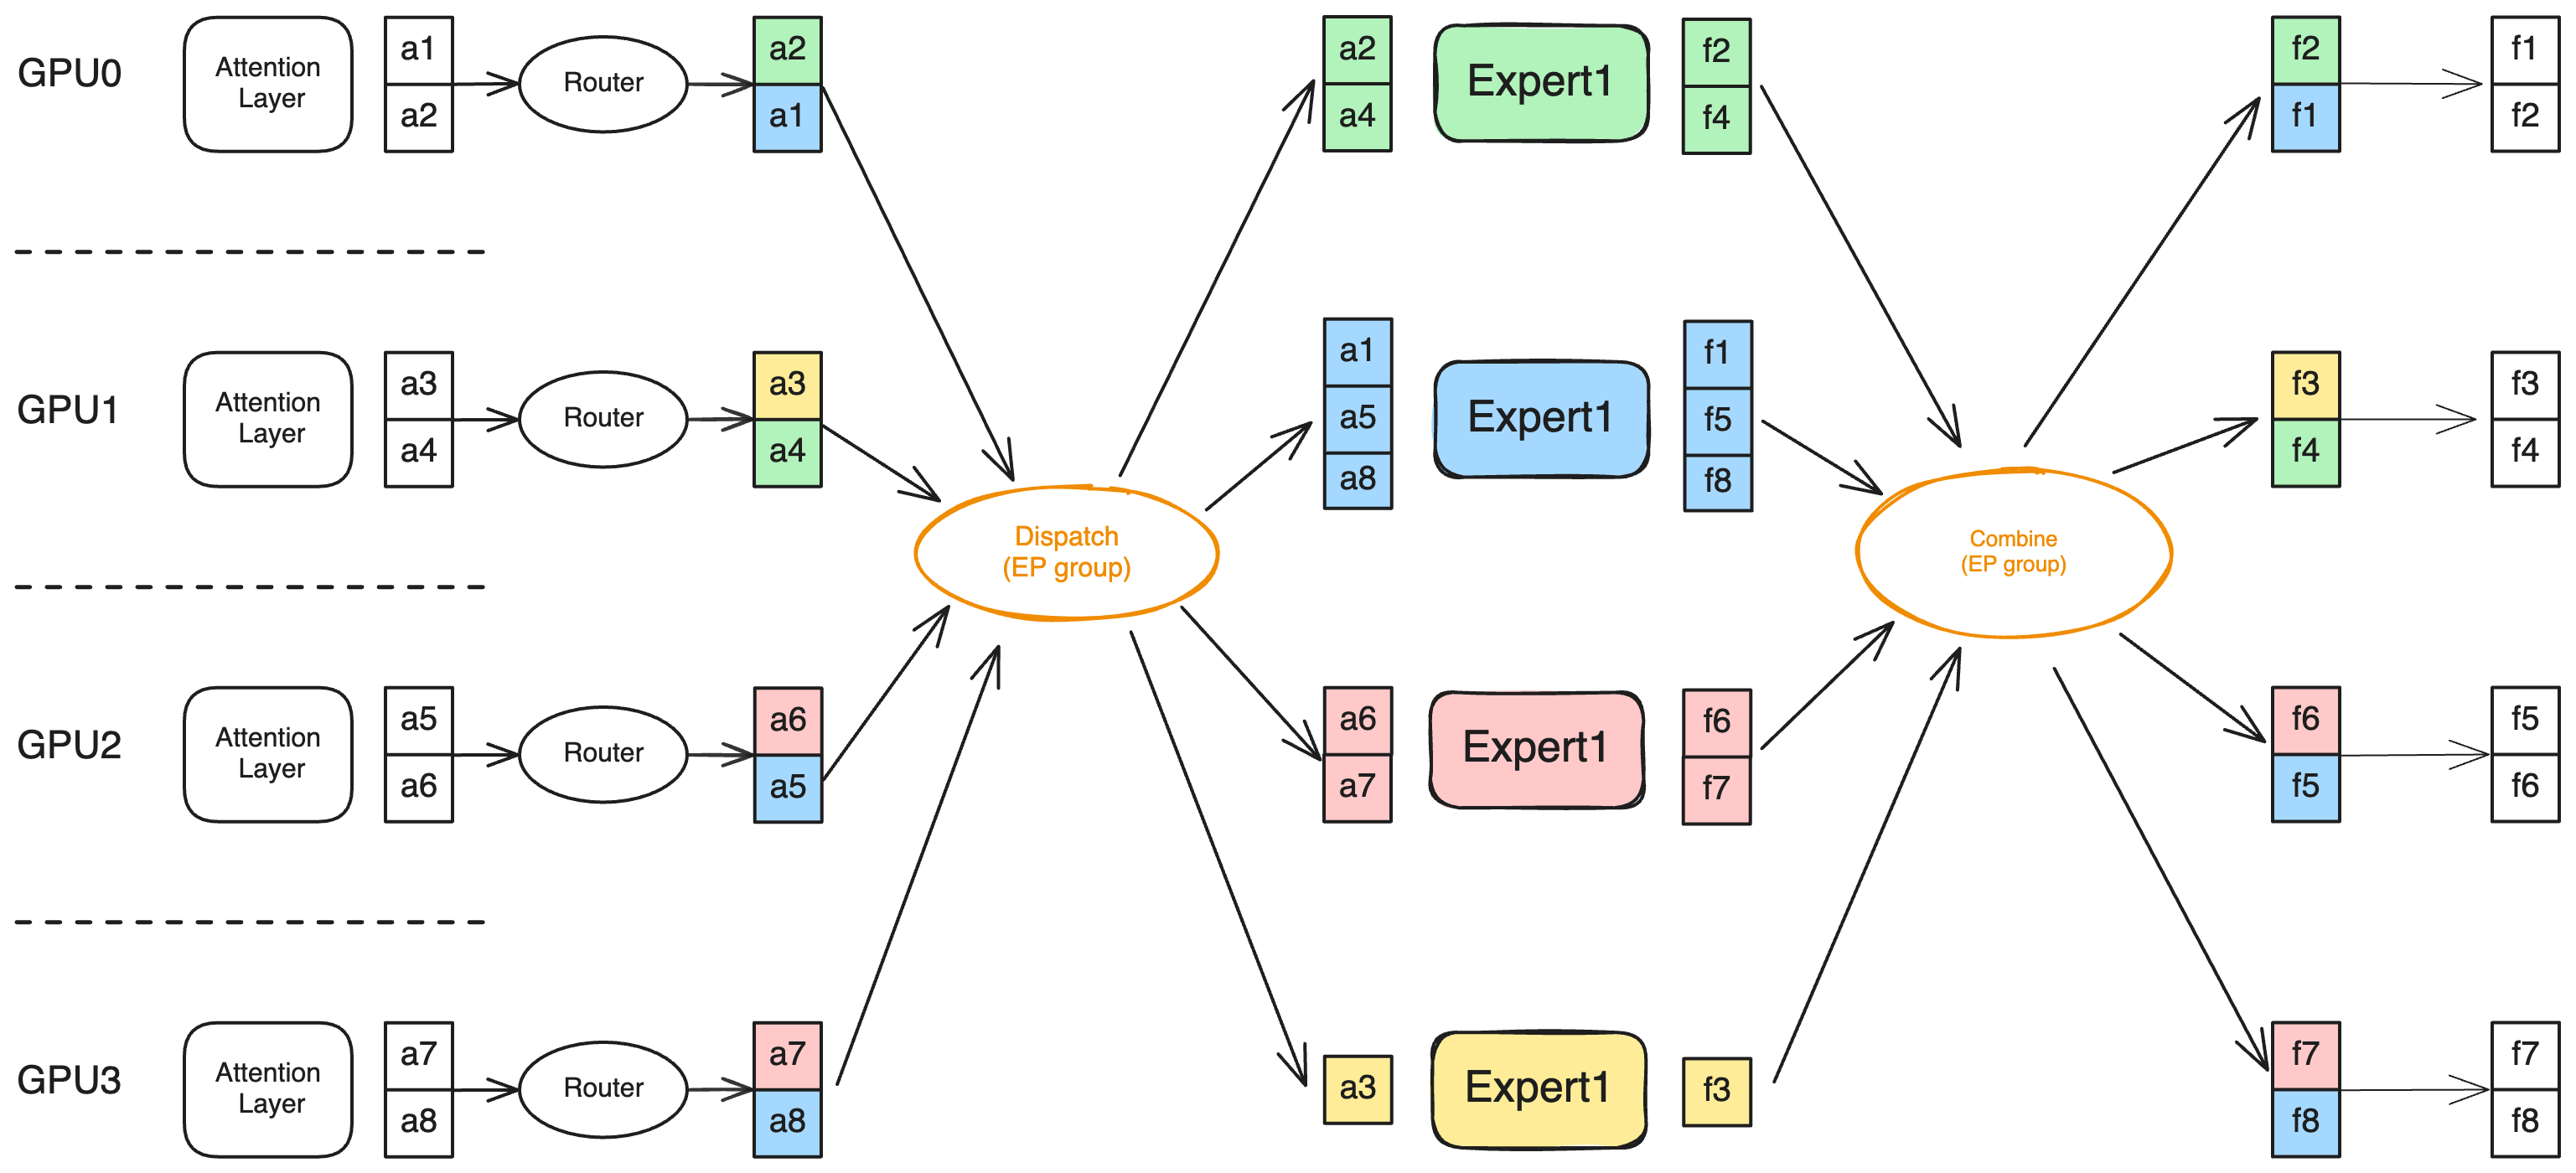
\includegraphics[width=0.8\linewidth]{figures/EP_comm.png}
    \caption{Expert parallelism across 4 GPUs with 4 experts.}
    \label{fig:EP_comm}
\end{figure}

\Figref{fig:EP_comm} illustrates the expert parallelism communication pattern. In standard EP implementations, each MoE layer requires two collective communication operations: \textit{dispatch} sends tokens to their assigned experts, and \textit{combine} returns processed tokens to their original ranks. For a model with $L$ MoE layers, $B$ tokens per batch, hidden dimension $h$, and EP degree $\text{EP}$, each forward pass involves $2L$ dispatch/combine operations, each transferring $O(Bh)$ data across $\text{EP}$ ranks.

At DeepSeek-V3 scale, this translates to 58 MoE layers $\times$ 2 operations/layer = 116 dispatch/combine operations per forward pass. The backward pass doubles this count. At 50 GB/s inter-node bandwidth (e.g., InfiniBand NDR), a single dispatch with 200 MB payload takes several milliseconds, accumulating to hundreds or thousands of milliseconds per iteration.

Communication volume is determined by the EP configuration and cannot be reduced without changing the parallelism strategy. Optimization must therefore target how communication is executed and scheduled. Two strategies work together to address communication overhead:

\begin{enumerate}
    \item \textbf{Maximize bandwidth utilization.} Standard NCCL all-to-all implementations do not fully exploit available bandwidth, particularly for fine-grained MoE workloads. Optimized dispatchers (DeepEP, HybridEP) use specialized kernels that fuse operations and exploit hardware primitives to approach peak bandwidth.
    \item \textbf{Hide latency behind computation.} Even with optimal bandwidth, all-to-all operations take time. By overlapping communication with computation from adjacent microbatches, this latency can be hidden rather than exposed on the critical path.
\end{enumerate}

The following subsections present techniques organized by these strategies: bandwidth optimization (DeepEP, HybridEP), and latency hiding (EP communication overlapping, pipeline integration).

\subsubsection{DeepEP and HybridEP: Maximizing EP Bandwidth}\label{sec:deepep}

In conventional EP implementations, token exchange relies on all-to-all communication. Even with optimized NCCL collectives, this path has inherent limitations: a permutation stage is needed before dispatch, which replicates each token top-$k$ times and creates redundant traffic. In some settings, this preprocessing also surfaces as host overhead.

To address these issues, Megatron-Core provides two token-based dispatch backends, HybridEP and DeepEP \cite{deepep2025}. Token-based dispatch eliminates the permutation step and avoids sending redundant tokens, reducing overall communication volume and improving effective bandwidth.

HybridEP was developed by NVIDIA. It follows the same token-based principle as DeepEP, exploits hardware primitives such as TMA and IBGDA, and targets comparable or higher bandwidth with lower SM usage, including Multi-Node NVLink (MNNVL) deployments.


\begin{figure}[ht]
    \centering
    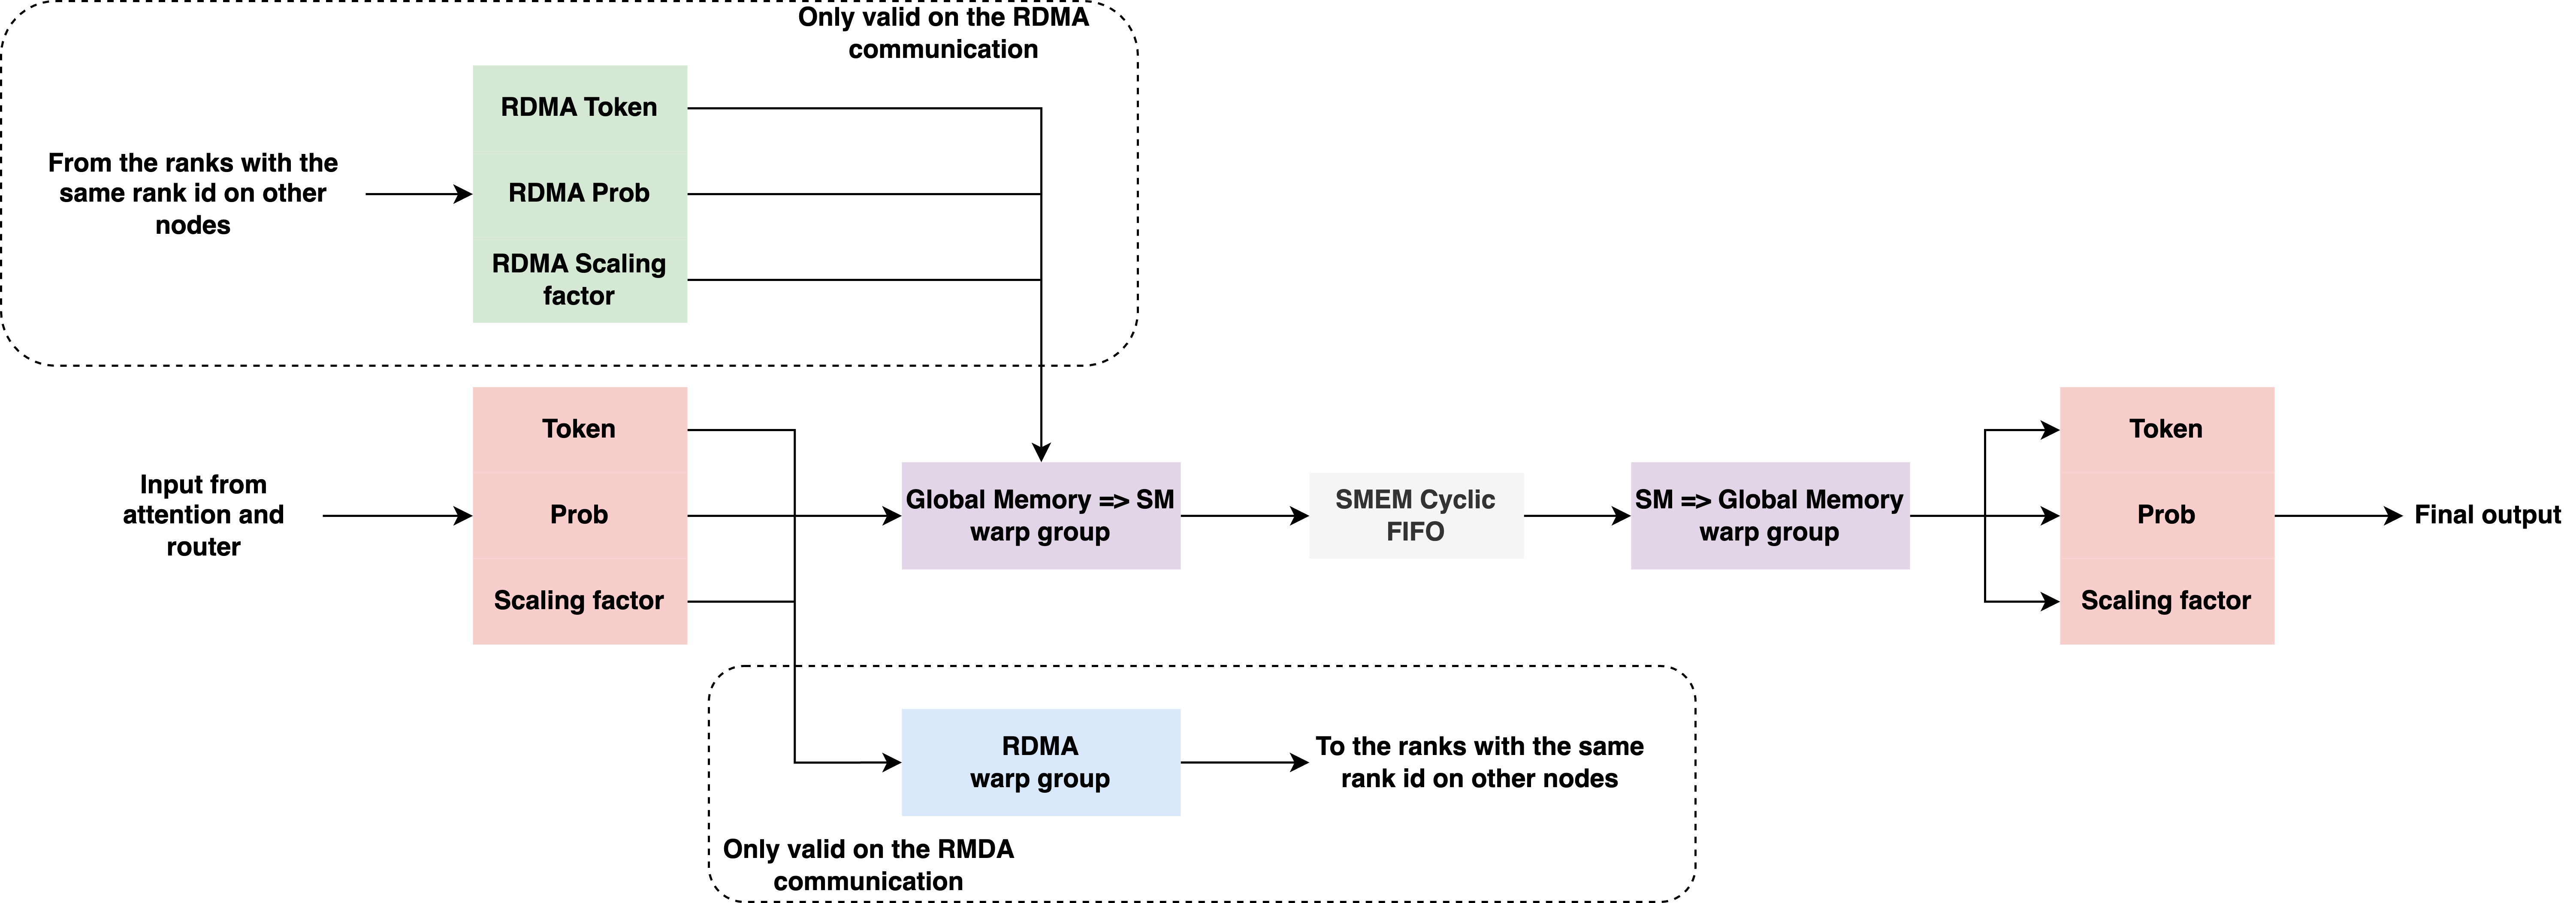
\includegraphics[width=1\linewidth]{figures/hybrid_ep_dispatch.drawio.png}
    \caption{The dispatch kernel design of HybridEP.}
    \label{fig:hybrid_ep_dispatch}
\end{figure}

For dispatch, as illustrated in \figref{fig:hybrid_ep_dispatch}, HybridEP reads data from global memory into shared memory based on routing information, then writes tokens to destinations through a FIFO queue. In the inter-node case, instead of sending duplicated payloads directly through the network interface, HybridEP first uses an RDMA warp group to exchange data between GPUs with the same local index across nodes, then forwards within each node. This reduces cross-node traffic and allows inter-node and intra-node transfers to overlap.

\begin{figure}[ht]
    \centering
    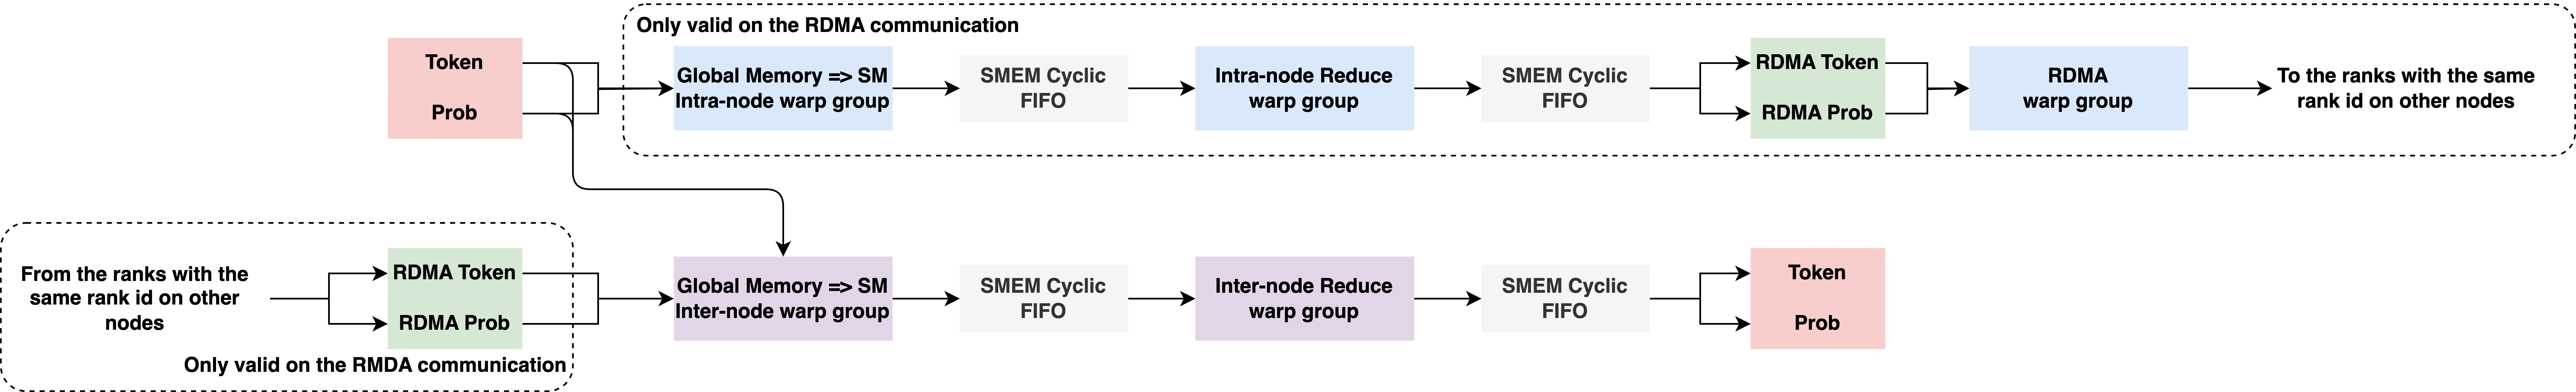
\includegraphics[width=1\linewidth]{figures/hybrid_ep_combine.drawio.png}
    \caption{The combine kernel design of HybridEP.}
    \label{fig:hybrid_ep_combine}
\end{figure}

For combine, standard all-to-all dispatch performs communication only, so a separate unpermutation stage is required afterward. HybridEP instead fuses reduction into the communication kernel. As shown in \figref{fig:hybrid_ep_combine}, HybridEP reads data through a FIFO queue, performs reduction, and writes results directly to target locations. In inter-node settings, HybridEP first performs reduction across nodes for data that must be communicated cross-node, then completes a second reduction within each node.


We evaluate all-to-all dispatch and HybridEP on GB200 and H100 with hidden size 7168, sequence length 4096, and 256 experts under multiple EP sizes. Results are summarized in Table~\ref{tab:hybrid-ep}. Across all tested settings, HybridEP consistently outperforms all-to-all, with larger gains in inter-node scenarios. The table reports communication latency only; in end-to-end training, the gap is typically larger once permutation and host overhead are included.

\begin{table}[ht]
\centering
\caption{EP Scaling Performance for HybridEP and all-to-all (in µs).}
\label{tab:hybrid-ep}
\begin{tabular}{llrrrr}
\toprule
 &  & \multicolumn{2}{c}{GB200 (µs)} & \multicolumn{2}{c}{H100 (µs)} \\
 & EP size & HybridEP & all-to-all & HybridEP & all-to-all \\
\midrule
\multirow{4}{*}{dispatch}
 & 8  & 391 & 735 & 661  & 1265 \\
 & 16 & 578 & 743 & 1485 & 5774 \\
 & 32 & 612 & 769 & 3064 & 8059 \\
 & 64 & 675 & 930 & 4626 & 9164 \\
\midrule
\multirow{4}{*}{combine}
 & 8  & 353 & 741 & 624  & 1277 \\
 & 16 & 527 & 765 & 1688 & 5628 \\
 & 32 & 646 & 758 & 3088 & 7815 \\
 & 64 & 744 & 827 & 4398 & 8727 \\
\bottomrule
\end{tabular}
\end{table}



\subsubsection{EP Communication Overlapping: Hiding EP Communication Latency}\label{sec:comm-overlap}

Optimized dispatchers improve all-to-all \textit{bandwidth utilization}, but the fundamental issue remains: all-to-all still lies on the end-to-end critical path. For DeepSeek-V3 with EP64, EP all-to-all communication can still account for 30--40\% of iteration time, directly limiting throughput.

The key observation is that all-to-all latency can be \textit{hidden} behind computation when enough independent work exists in the overlap window \cite{wang2022coconet,wang2024flux}. For fine-grained MoE models such as DeepSeek-V3 and Kimi-K2, this is challenging because cross-node EP communication can consume about half of layer time, while adjacent operators (for example, GEMMs) are often too short to hide it.

To address this imbalance, Megatron-Core uses a dedicated 1F1B all-to-all overlap scheme \cite{1f1boverlap} that merges forward and backward passes from neighboring micro-batches and interleaves compute and all-to-all kernels across CUDA streams \cite{narayanan2019pipedream,huang2019gpipe}. Concretely, backward all-to-all for one micro-batch overlaps with forward attention/MLP for another. Conceptually, this is a DualPipe-like \cite{hfdualpipe} bidirectional schedule built on top of standard 1F1B while preserving Megatron-Core compatibility.

To enable all-to-all overlap in 1F1B, we merge adjacent micro-batch forward and backward passes and evaluate two patterns:

\begin{enumerate}
    \item \textbf{Merged FWD-FWD / BWD-BWD}: This strategy merges passes of the same type from two micro-batches (\figref{fig:fwd_fwd_merge}). In \textit{FWD-FWD}, forward passes for micro-batches 0 and 1 run in parallel and overlap all-to-all with computation. \textit{BWD-BWD} applies the same principle to backward passes. This approach has clear trade-offs:
    \begin{itemize}[leftmargin=*]
        \item \textbf{Memory Overhead}: 2x peak activation memory.
        \item \textbf{all-to-all Overlap}: Less opportunity to hide all-to-all because forward computation is roughly half of backward computation.
    \end{itemize}
    
    \begin{figure}[ht]
        \centering
        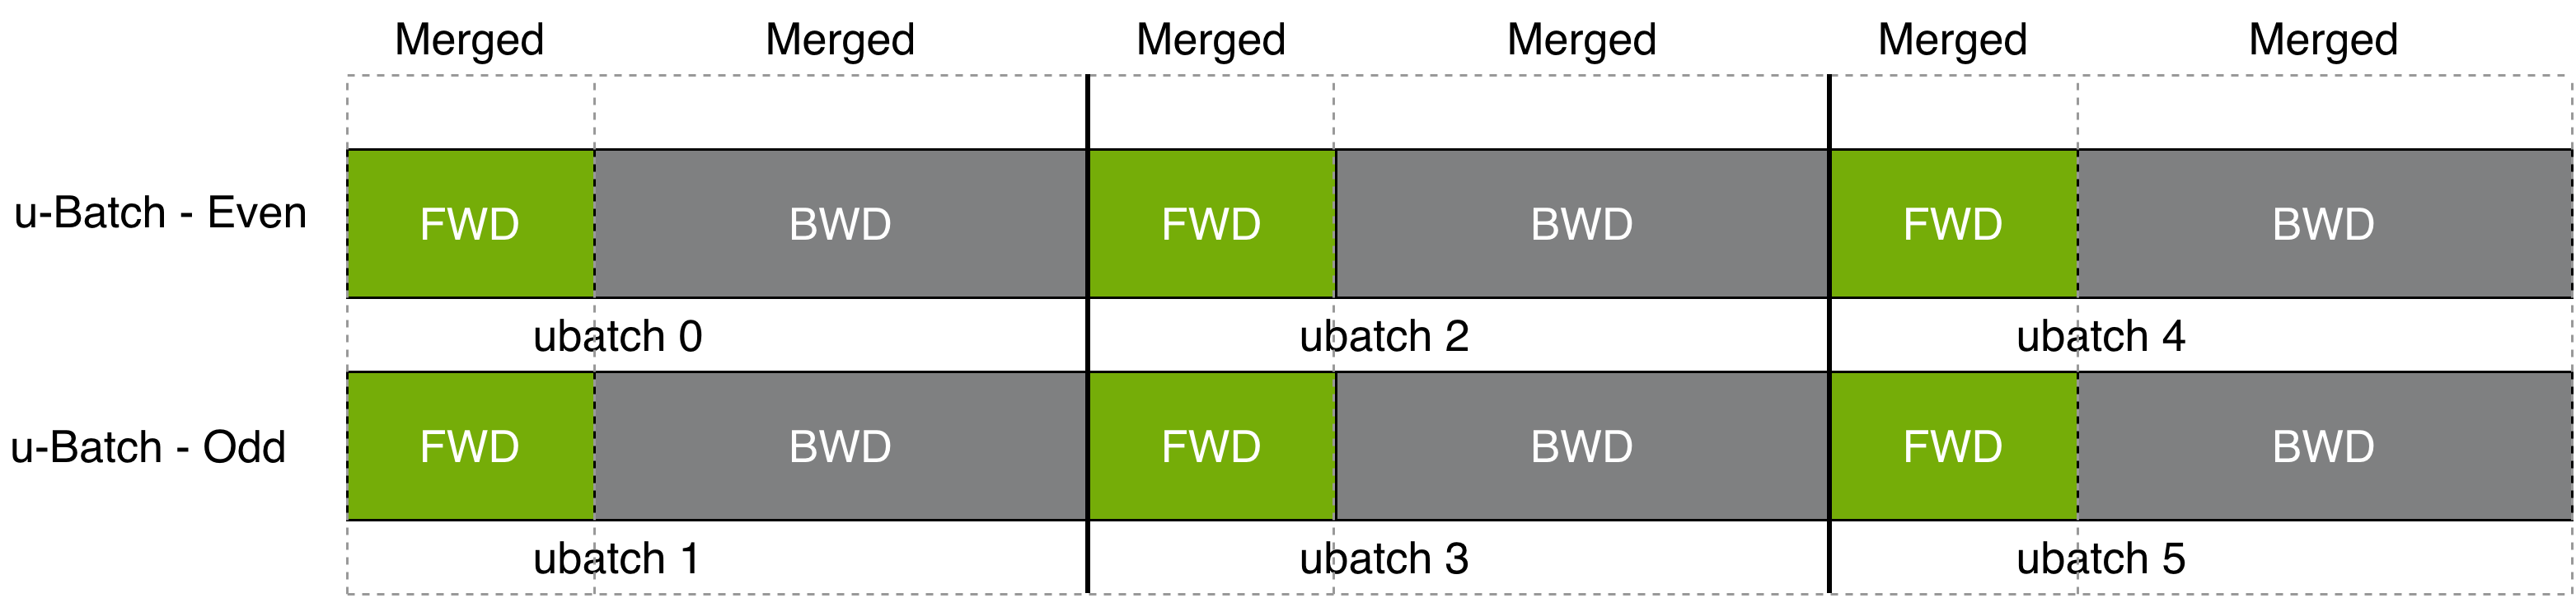
\includegraphics[width=0.8\linewidth]{figures/EP_Overlap_merged_fwd_fwd.png}
        \caption{Merged FWD-FWD Timeline with all-to-all Overlapping.}
        \label{fig:fwd_fwd_merge}
    \end{figure}

    \item \textbf{Merged FWD-BWD (DualPipe Equivalent)}: This is the preferred strategy (\figref{fig:fwd_bwd_merge}). It merges the forward pass of one micro-batch with the backward pass of another (for example, FWD of micro-batch 1 with BWD of micro-batch 0). Compared with \textit{FWD-FWD}, it offers:
    \begin{itemize}[leftmargin=*]
        \item \textbf{Memory Overhead}: No additional memory overhead (activations from the forward pass are reused for the backward pass).
        \item \textbf{Compatibility}: Matches DualPipe's design but avoids complex scheduling.
        \item \textbf{Limitation}: The first FWD and last BWD remain on the end-to-end critical path, so their all-to-all cannot be hidden.
    \end{itemize}

    
    \begin{figure}[ht]
        \centering
        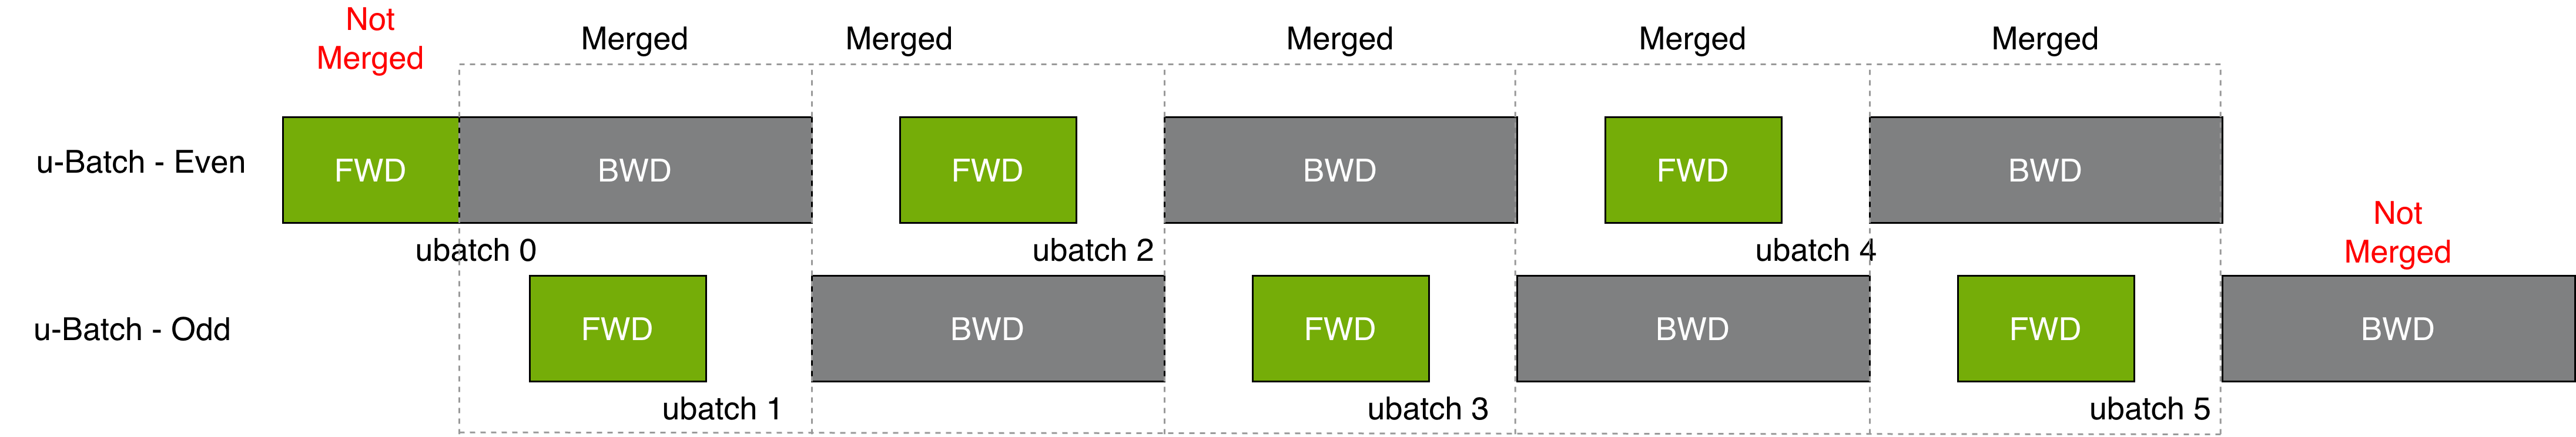
\includegraphics[width=0.8\linewidth]{figures/EP_Overlap_merged_fwd_bwd.png}
        \caption{Merged FWD-BWD Timeline with all-to-all Overlapping.}
        \label{fig:fwd_bwd_merge}
    \end{figure}
\end{enumerate}

To maximize all-to-all hiding in merged FWD-BWD, we use two key optimizations:

\begin{enumerate}
    \item \textbf{Stream Separation}: We split workloads into two CUDA streams:
    \begin{itemize}[leftmargin=*]
        \item \textit{Compute Stream}: Runs forward/backward computations (e.g., attention, expert MLP).
        \item \textit{Comm Stream}: Runs all-to-all communication (e.g., token dispatch/combine for EP).
    \end{itemize}
    By alternating tasks across streams, all-to-all runs in parallel with computation—minimizing idle cycles.

    \item \textbf{W/D Split (Weight-Gradient / Data-Gradient Split)} \cite{deepseekai2025deepseekv3technicalreport}: A key dependency blocks overlap: backward dispatch (B/dispatch) requires outputs from backward MLP (B/mlp). To break this dependency, we split backward MLP into:
    \begin{itemize}[leftmargin=*]
        \item \textit{W/mlp}: Weight gradient calculation (independent of B/dispatch).
        \item \textit{D/mlp}: Data gradient calculation (feeds into B/dispatch).
    \end{itemize}
    This split reduces compute-stream idle time: W/mlp can overlap with F/mlp to hide B/dispatch when F/mlp alone is too short.
\end{enumerate}
\Figref{fig:ep-all-to-all-overlap} summarizes these optimizations. The baseline (top) executes sequentially, where all-to-all blocks computation. The 1F1B FWD-BWD scheme (bottom) interleaves adjacent micro-batches so communication can be hidden behind compute. The W/D split further increases overlap opportunities. Together, these methods reduce EP communication overhead from 30--40\% (after DeepEP) to under 5\% of iteration time in DeepSeek-V3 training on H100.

\begin{figure}[ht]
    \centering
    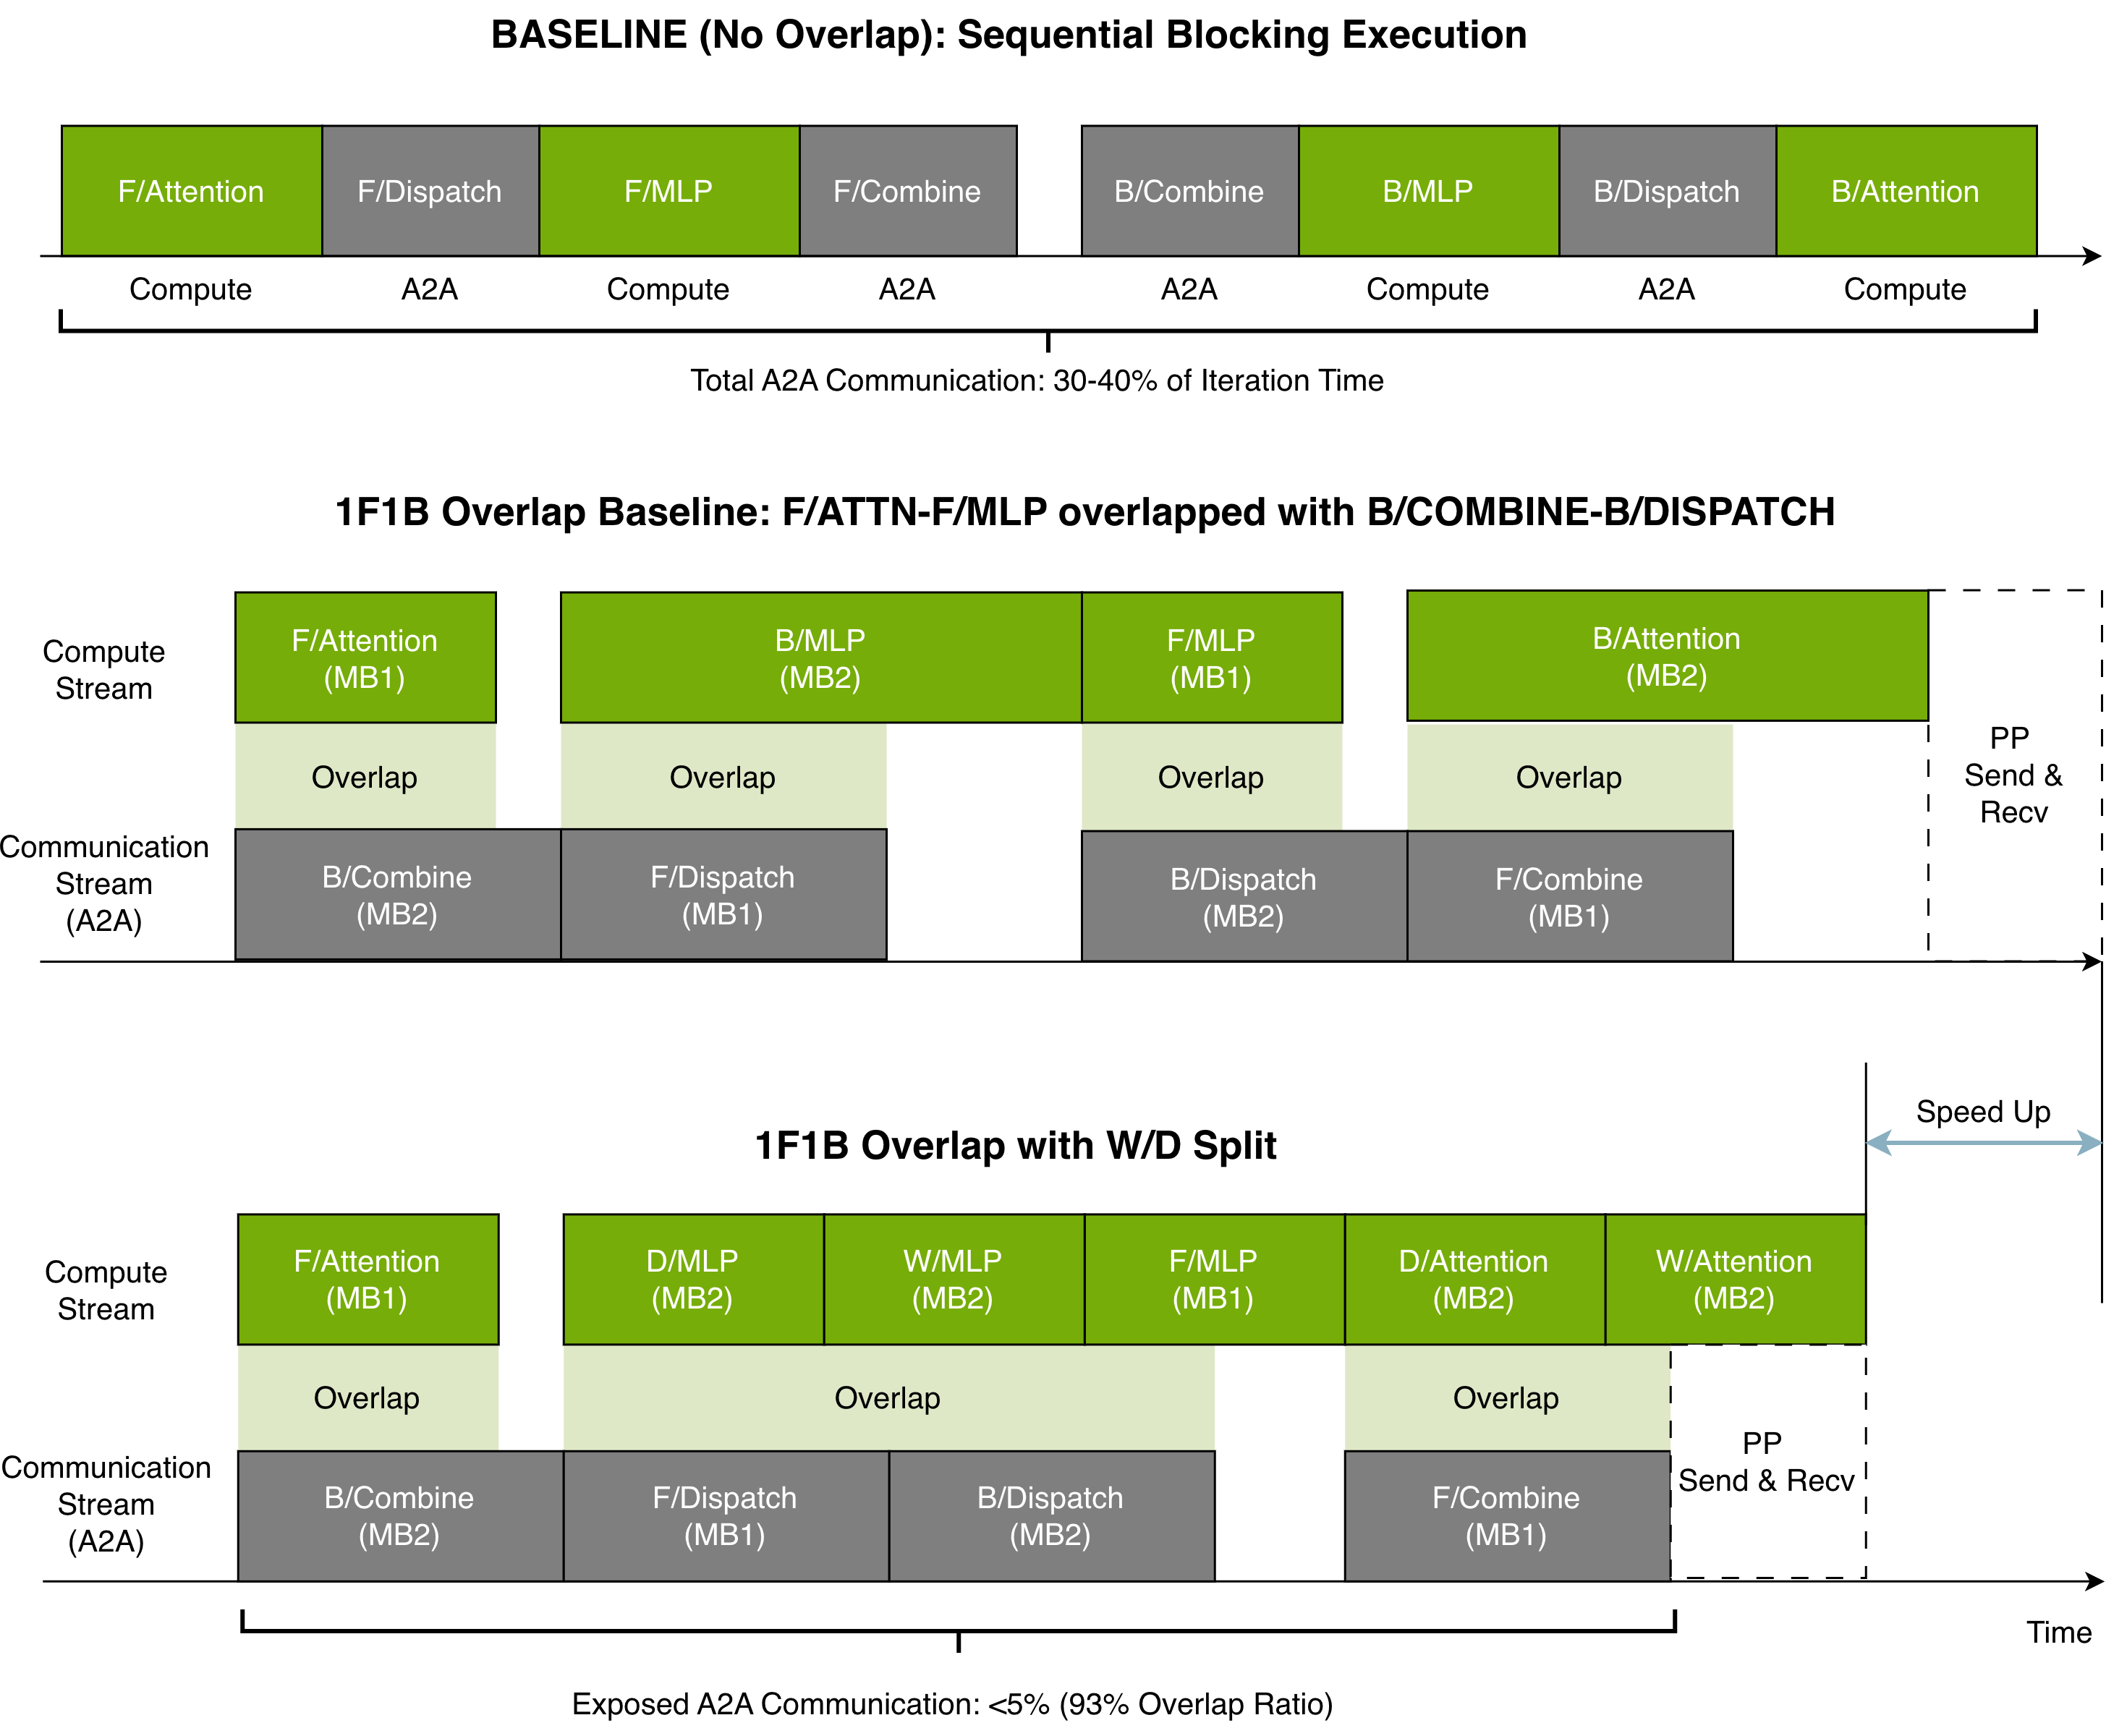
\includegraphics[width=0.9\textwidth]{figures/EP_Overlap_Summary.png}
    \caption{EP all-to-all communication overlap strategies: baseline vs. 1F1B with W/D split.}
    \label{fig:ep-all-to-all-overlap}
\end{figure}

% \begin{figure}[ht]
%     \centering
%     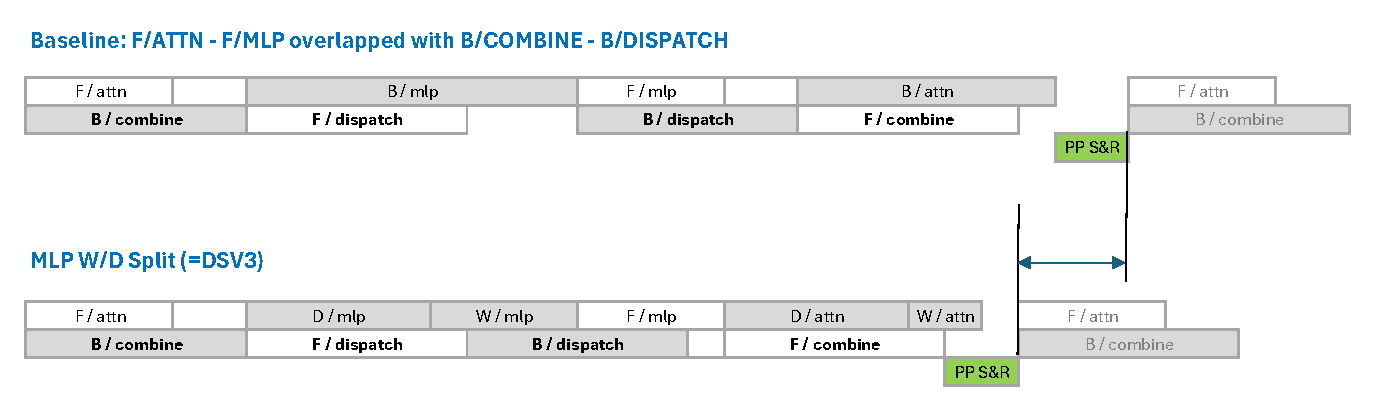
\includegraphics[width=0.8\linewidth]{figures/1f1b_split_wgrad.pdf}
%     \caption{Compute/Comm Stream Schedules}
%     \label{fig:compute_comm_streams}
% \end{figure}

To scale overlap to large models, merged FWD-BWD can be combined with \textit{Interleaved Pipeline Parallelism} (Interleaved PP), which partitions the model into virtual pipeline stages (VPP) and expands overlap opportunities across pipeline ranks. \Figref{fig:interleaved_pp} shows an interleaved 1F1B schedule with three phases: warmup, 1F1B, and flush. Adjacent FWD-BWD pairs in the 1F1B phase can apply the EP overlap pattern above. However, adjacent pairs may still have data dependencies when they belong to the same micro-batch. To avoid this, we run \textit{one extra micro-batch} at the end of warmup before entering 1F1B, ensuring adjacent FWD/BWD pairs are dependency-free and enabling full all-to-all overlap across virtual stages.

A latency comparison between merged FWD-BWD (1F1B) and DualPipeV (a refined DualPipe variant) shows:
\begin{itemize}
    \item \textit{1F1B is faster} with large VPP sizes (more virtual stages enable more overlapping opportunities).
    \item The latency gap shrinks at large PP sizes and micro-batch counts (both strategies reach near-optimal overlap).
    \item For hybrid models (e.g., DeepSeek-V3 with mixed dense/MoE layers), workload balance across PP stages is critical. Megatron-Core's \textit{Flexible Asymmetric VPP} supports custom per-stage layer placement to maximize overlap.
\end{itemize}

\begin{figure}[ht]
    \centering
    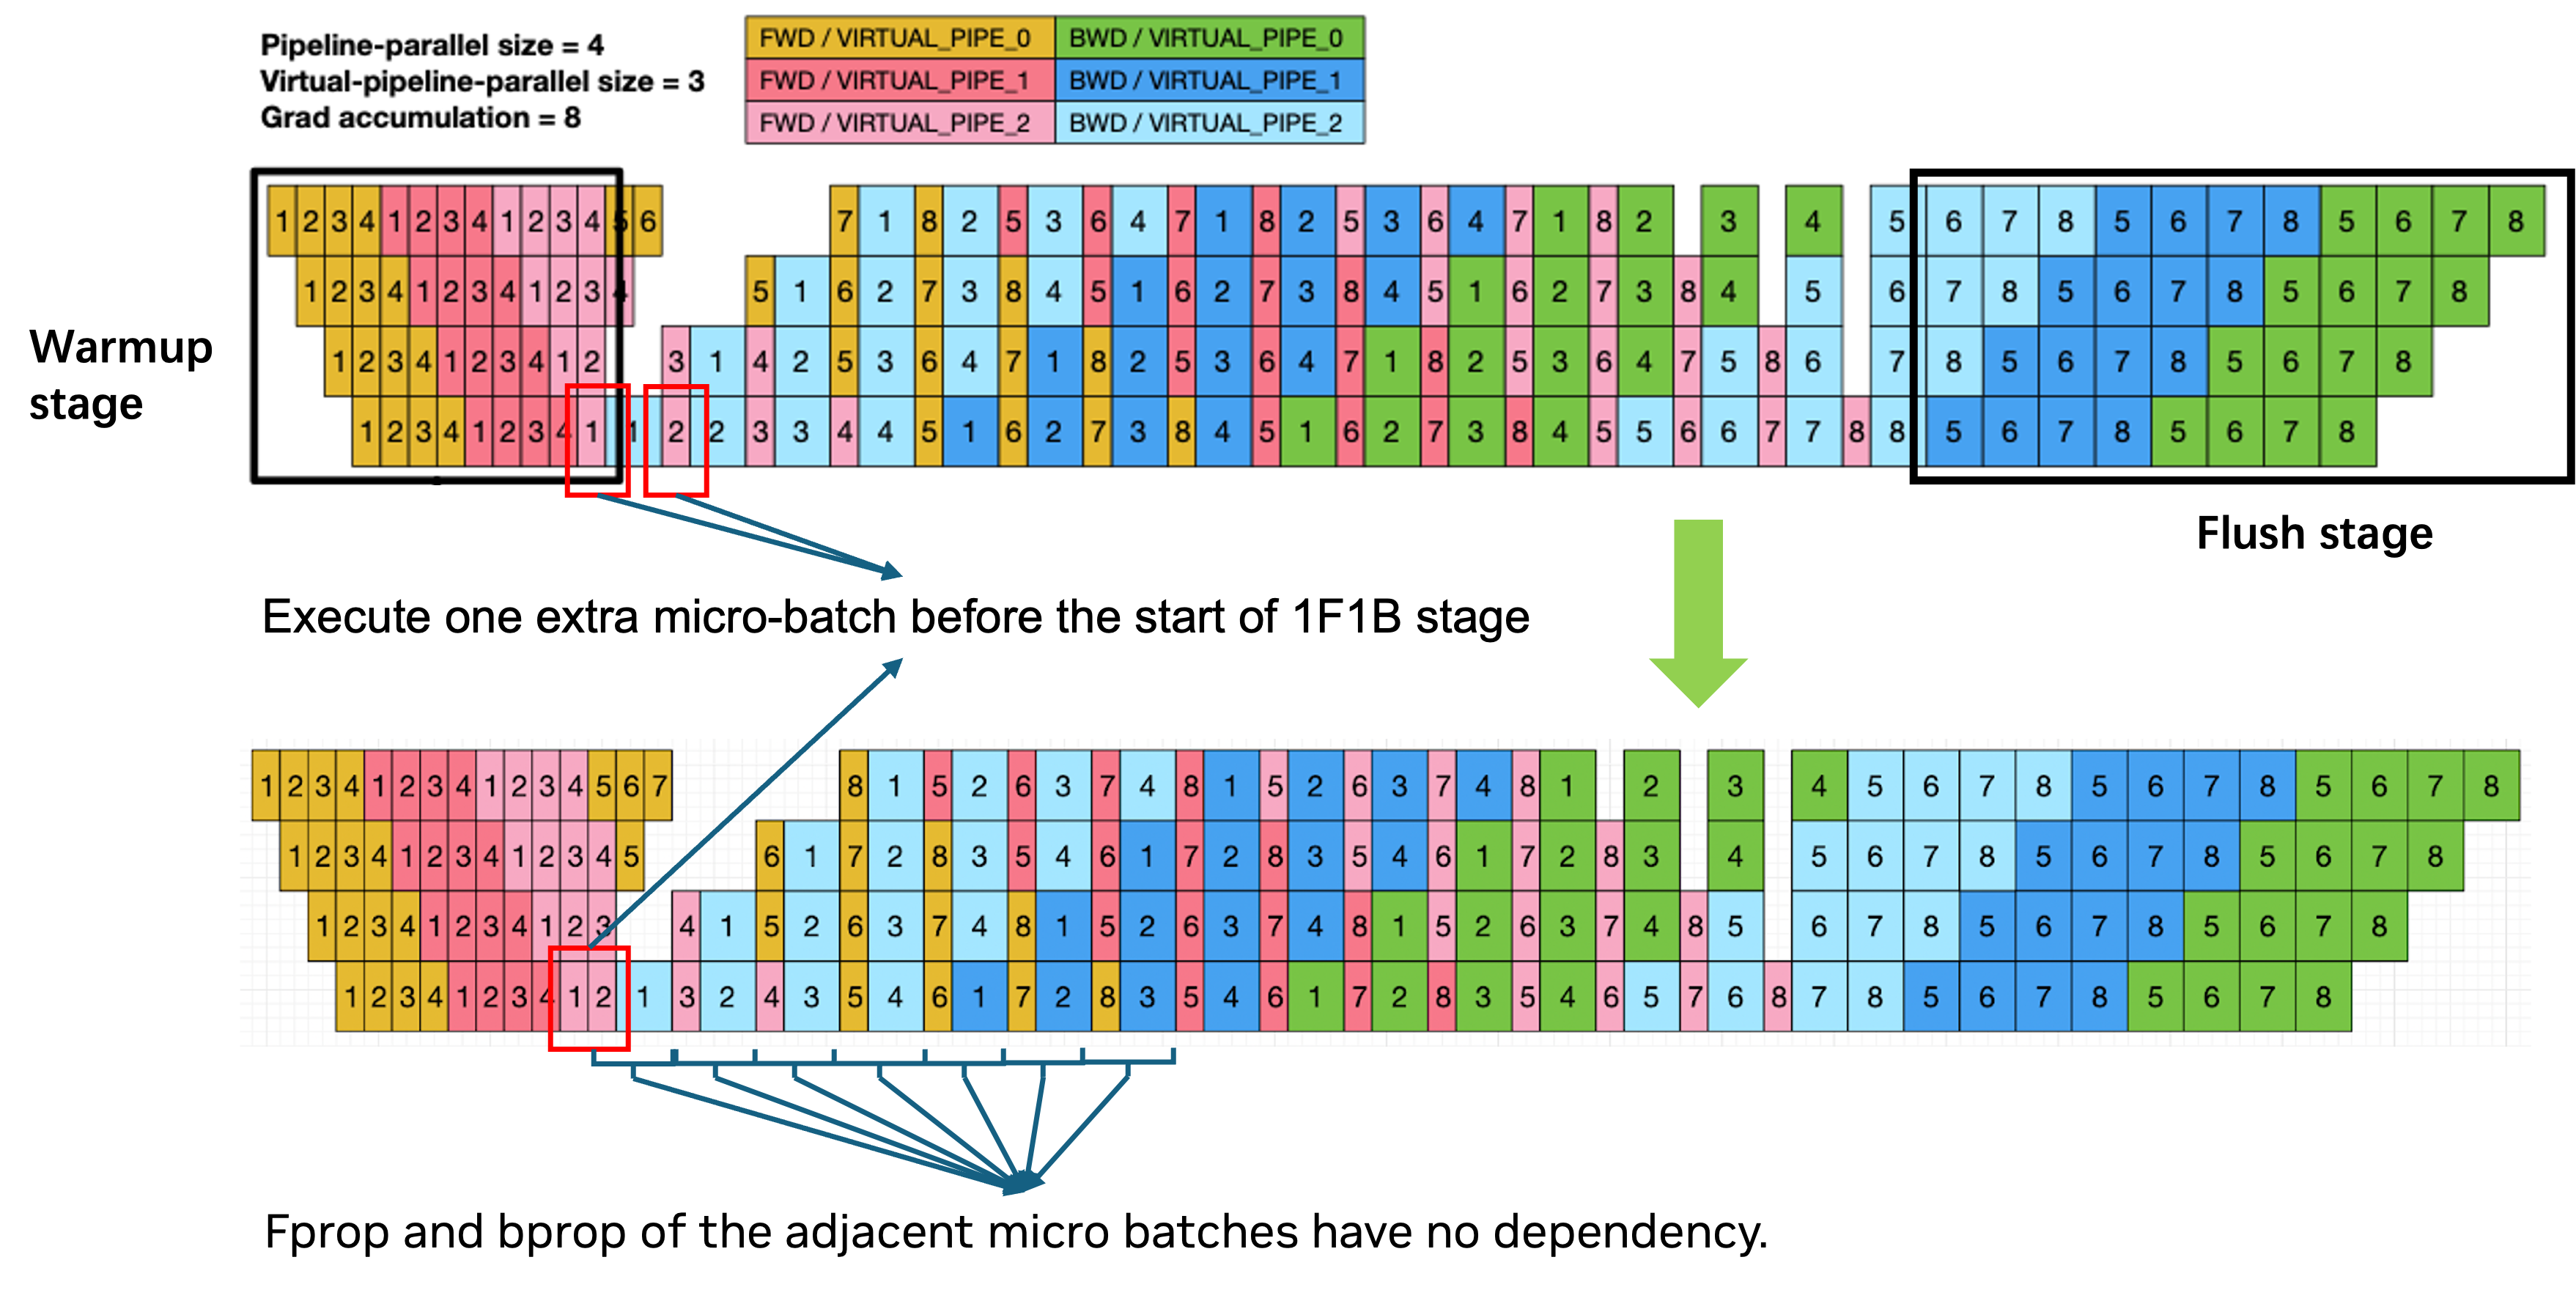
\includegraphics[width=0.9\linewidth]{figures/interleaved_pp.png}
    \caption{Interleaved PP Timeline with all-to-all Overlapping.}
    \label{fig:interleaved_pp}
\end{figure}

Several factors limit the achievable speedup from all-to-all overlap:
\begin{itemize}
    \item \textbf{Proportion of overlapped batches}: More micro-batches increase the proportion of overlapped batches.
    \item \textbf{all-to-all Proportion}: EP overlap gains are larger when all-to-all dominates, especially for cross-node EP and fine-grained MoE models with low compute-to-communication ratios.
    \item \textbf{SM Carve-out Overhead}: Reserving SMs for all-to-all can reduce GEMM efficiency. In our DeepSeek-V3 benchmark, DeepEP uses 20 SMs per GPU and introduces roughly 20\% GEMM-efficiency overhead.
\end{itemize}

On fine-grained MoE models such as DeepSeek-V3, combining all-to-all overlap with optimized dispatchers (Section~\ref{sec:deepep}) achieves a 93\% overlap ratio for expert communication latency, reducing expert communication share from 30--40\% of iteration time to under 5\%.


% \subsubsection{FP8 EP Communications: Reducing Communication Volume}\label{sec:fp8-comm}

% The optimizations above hide all-to-all latency behind computation. An orthogonal approach is to reduce the all-to-all \textit{volume} itself. By performing dispatch communication in FP8 instead of BF16, we halve the data transferred per all-to-all operation.

% However, FP8 dispatch requires careful handling depending on the FP8 recipe:
% \begin{itemize}
%     \item \textbf{Blockwise/Subchannel FP8}: Tokens must be quantized before dispatch. In backward pass, we dequantize to reconstruct high-precision input, then re-quantize because forward and backward use different quantization dimensions. Transposition may be required for Hopper Tensor Core layouts.
%     \item \textbf{MXFP8}: Similar to blockwise, though transposition is unnecessary as Blackwell Tensor Cores accept any layout, backward computation requires the input tokens to be quantized along a different dimension. As a result, dequantization and re-quantization are still needed.
% \end{itemize}

% Note that \textit{combine} communication typically remains in higher precision to avoid gradient accumulation errors. The dispatch-only FP8 strategy provides 50\% all-to-all volume reduction with minimal accuracy impact. See Section~\ref{sec:fp8-dispatch-comm} for more details.

\subsubsection{Summary}
The communication wall optimizations work together: DeepEP/HybridEP maximize bandwidth utilization; FWD-BWD overlap hides latency behind computation; Interleaved PP extends overlap opportunities across pipeline stages; Flexible VPP enables optimal load balance. Combined, they reduce all-to-all's contribution to training time under 10\%.

With communication latency hidden behind computation, high GPU utilization might be expected. However, profiling reveals the Compute Efficiency Wall, which has two distinct aspects: \textit{kernel efficiency} (fine-grained experts produce small GEMMs that underutilize GPU resources) and \textit{host overhead} (numerous small operations create gaps between kernel executions where the GPU awaits work from the host).

\subsection{Breaking the Compute Efficiency Wall}\label{sec:compute-wall}

Compute efficiency is the final constraint: even with sufficient memory and hidden communication, GPU resources can remain underutilized if kernels are inefficient or the host cannot dispatch work fast enough. As model and expert counts grow, compute inefficiencies compound, making optimization essential for achieving peak hardware utilization.

\subsubsection{Compute Anatomy: Sources of Inefficiency}

Compute inefficiency in MoE training stems from two distinct sources:

\textbf{Kernel Efficiency.} Fine-grained MoE architectures produce workloads that underutilize GPU resources. DeepSeek-V3's 256 small experts yield GEMMs with M dimensions of $\sim$128 tokens per expert, far from the thousands needed for peak Tensor Core utilization. Beyond expert computation, MoE introduces complex routing and dispatching operations composed of many small kernels that individually cannot saturate GPU compute capacity.

\textbf{Host Overhead.} Numerous small operations create kernel launch overhead, and the CPU cannot dispatch work fast enough to keep the GPU saturated. Three factors make this worse:
\begin{itemize}
    \item \textbf{Fine-grained experts}: Many individual GEMMs rather than few large ones, each requiring a separate kernel launch.
    \item \textbf{Reduced-precision training}: Additional quantization kernels add to the launch overhead.
    \item \textbf{Dropless routing}: Dynamic token counts require host-device synchronization to determine tensor shapes, placing the CPU on the critical path.
\end{itemize}

The result is \textit{host-boundedness}: GPU kernels separated by microseconds of host-side latency, visible as gaps in profiling traces where compute resources sit idle.

Kernel shapes are determined by model architecture and cannot be changed without modifying the model. Optimization must therefore target how computation is organized and scheduled. Five strategies work together to address compute inefficiency:

\begin{enumerate}
    \item \textbf{Fuse related operations.} Kernel fusion consolidates routing, permutation, and auxiliary loss computations into fewer, larger kernels.
    \item \textbf{Accelerate with low precisions.} Reduced-precision training in FP8/FP4 uses faster Tensor Core operations, increasing throughput for the same kernel shapes.
    \item \textbf{Eliminate per-iteration CPU logic.} CUDA Graphs capture kernel sequences and replay them with minimal host involvement.
    \item \textbf{Remove host-device synchronization.} Sync-free execution enables GPU kernels to proceed without waiting for shape information from the host.
    \item \textbf{Balance expert load.} ECHO dynamically clones hot experts to underutilized ranks, reducing load imbalance that causes some ranks to wait while others compute.
\end{enumerate}

The following subsections present techniques organized by these strategies: batching and fusion for kernel efficiency (Section~\ref{sec:kernel-fusion}), low-precision acceleration (Section~\ref{sec:fp8-training}), CUDA Graphs for host overhead elimination (Section~\ref{sec:cuda-graphs}), sync-free execution for dropless MoE (Section~\ref{sec:sync-free-moe}), and load balancing via ECHO (Section~\ref{sec:echo}).

\subsubsection{Grouped GEMM and Kernel Fusion: Improving Kernel Efficiency}\label{sec:kernel-fusion}

The most direct approach to improving kernel efficiency is combining small operations into larger ones. Grouped GEMM batches expert computations for better hardware utilization \cite{megablocks}, while kernel fusion consolidates routing and permutation operations into fewer kernels \cite{chen2018tvm}. Megatron-Core implements these optimizations at three levels: expert computation (Grouped GEMM), token routing (Permutation Fusion), and router logic (Router and Aux-Loss Fusion).

\paragraph{Grouped GEMM}\label{sec:grouped-gemm}

The computation of experts is essentially a series of independent GEMMs. Grouped GEMM improves performance over separate sequential GEMMs by overlapping the wave tail effect of kernels.

Megatron-Core provides two Grouped GEMM implementations:

\begin{itemize}
\item[i.] Multi-stream launch of cuBLASLt GEMMs.
By launching individual cuBLASLt GEMMs into multiple CUDA streams, they can overlap with each other. This method supports various precision and scaling modes, including BF16, per-tensor FP8, blockwise FP8, MXFP8, and NVFP4, with performance comparable to highly optimized Grouped GEMM implementations.

\item[ii.]\label{gmm:2} CUTLASS Grouped GEMM.
By fusing individual GEMMs into a single kernel, CUTLASS Grouped GEMM achieves better performance when the number of GEMMs is large. However, different precisions, scaling modes, and hardware platforms require individual development effort, and additional tuning is needed for different problem sizes. The current implementation in TE only supports BF16 on the Hopper platform.
\end{itemize}


Two additional implementations are under development:

\begin{itemize}
\item[iii.] cuBLASLt Grouped GEMM via \texttt{CUBLASLT\_BATCH\_MODE\_GROUPED}.
The cuBLASLt Grouped GEMM assumes the shape information on device and conducts the computation in one single kernel, which unblocks applying CUDA Graphs to the expert part. It covers all precisions and scaling modes with built-in heuristics, and is intended to supersede (i) and (ii) where supported.

\item[iv.] cuteDSL Grouped GEMM with fusions.
Grouped GEMM fused with activation functions, quantization (for the next layer), and scaling factor swizzling via cuteDSL. These kernels are optimized for MXFP8 and NVFP4~\cite{abecassis2025nvfp4} on the Blackwell platform, targeting the \texttt{fprop} GEMM of FC1 and \texttt{dgrad} GEMM of FC2. By consolidating expert computation, activation, and quantization into a single kernel, this approach significantly reduces kernel count and is compatible with CUDA Graphs.
\end{itemize}

\subsubsection{Permutation Fusion}

Currently, Grouped GEMM requires tokens assigned to the same expert to be stored contiguously (i.e., permuted tokens). If all-to-all collective communication is enabled, further permutation is necessary to ensure tokens assigned to each rank are grouped together. Implementing efficient permutation using native PyTorch is challenging, as it tends to launch many small kernels and incurs additional CPU overhead.

The permute fusion pipeline in the training workload (\figref{fig:permute_fusion}) consists of three stages:

\begin{figure}[ht]
    \centering
    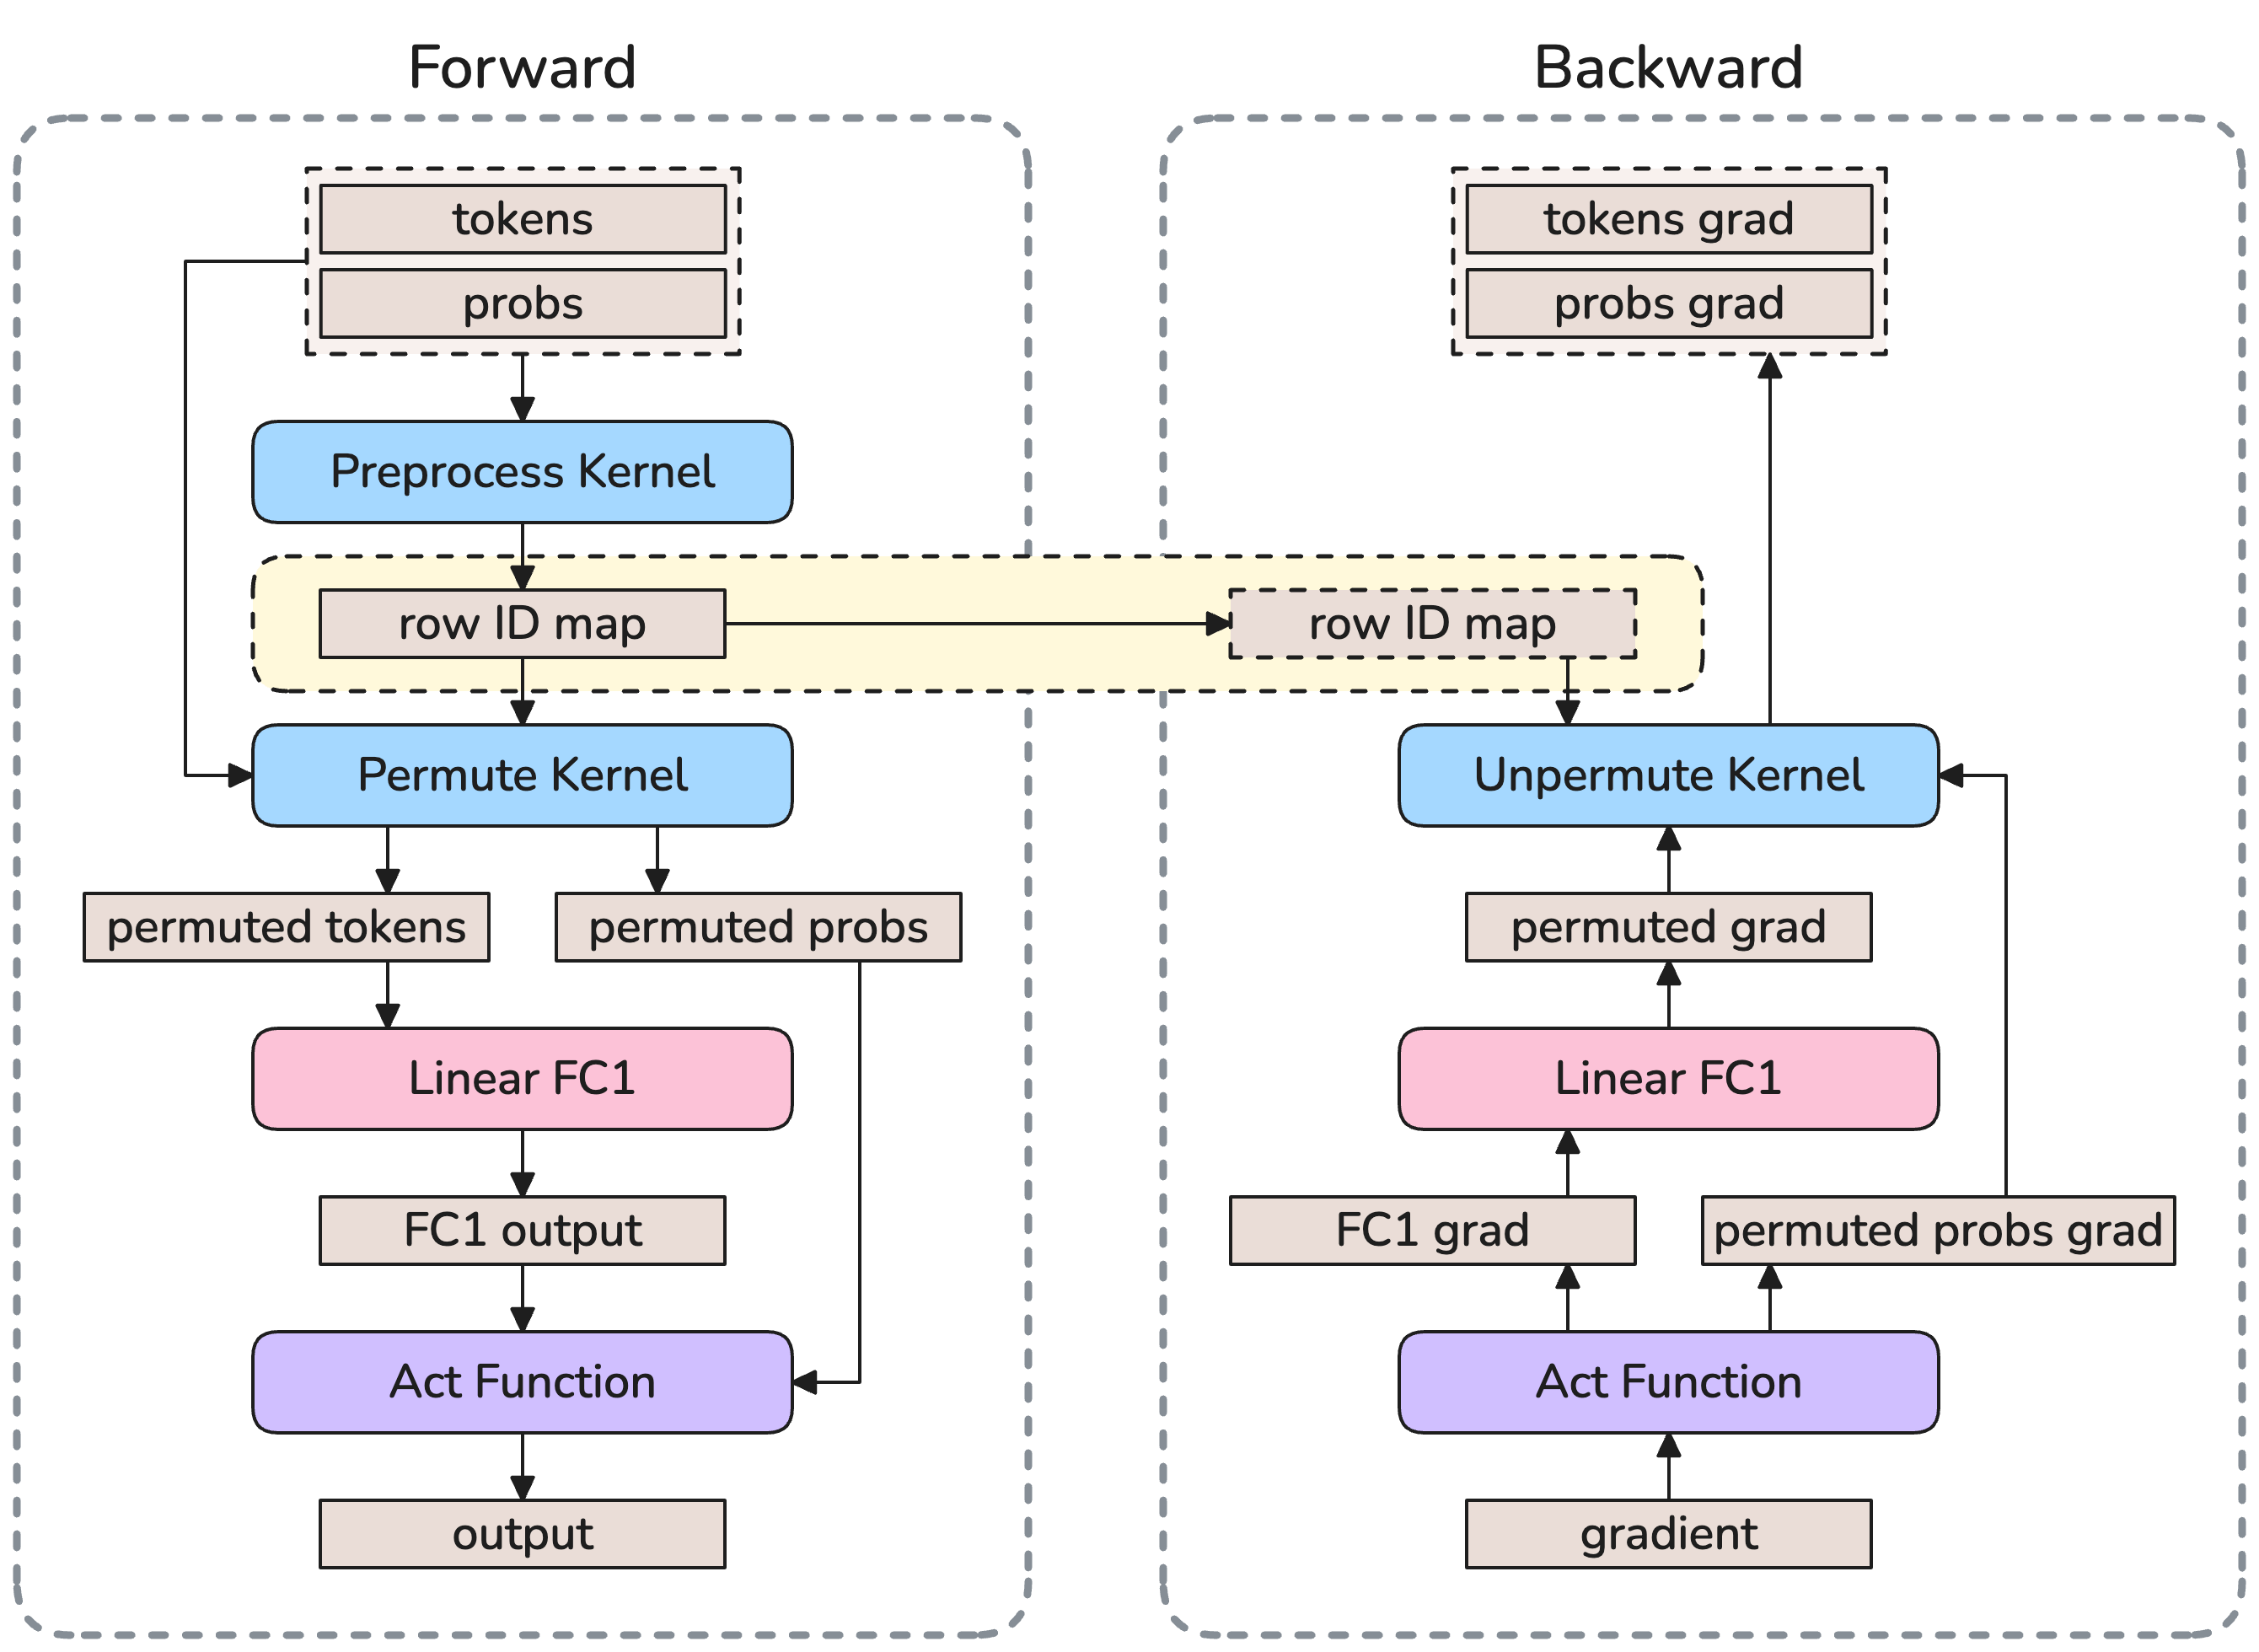
\includegraphics[width=0.6\linewidth]{figures/permute_fusion.png}
    \caption{The pipeline for permute fusion in the training process.}
    \label{fig:permute_fusion}
\end{figure}

\begin{itemize}
    \item Preprocessing: Permutation is fundamentally a data transfer process that requires tokens to be stored consecutively in the buffer corresponding to each expert. The purpose of the preprocessing step is to generate an offset map (Row ID map in \figref{fig:permute_fusion}), which indicates the offset of each token in the input and output buffers. This ensures that permute and unpermute operations can be executed efficiently. The preprocessing kernel is called only once before permute during the forward pass, while other components reuse the results.
    \item Permute: The functionality of the permute kernel is straightforward: it moves tokens from the input buffer to the output buffer according to the offset map, and then passes them to the subsequent expert MLP. In memory-efficient permute, probabilities also need to be permuted, with the results directly entering the activation part of the expert.
    \item Unpermute: The unpermute step is the inverse of the permute operation. Since a token will be copied multiple times and sent to different destinations during permutation, these tokens must be summed together during the combine phase. In memory-efficient permute, the combine step simply adds them up; otherwise, the probabilities are used as weights. All accumulation is performed in FP32 precision.
\end{itemize}

\subsubsection{Router and Aux-Loss Fusion}

The router and auxiliary loss \cite{fedus2022switchtransformersscalingtrillion,zoph2022stmoe,hwang2023tutel,rajbhandari2022deepspeedmoe} computations are other areas that generate many small kernels and introduce considerable CPU overhead. As device computing power grows, fusion becomes increasingly important.

The challenge is that the router contains components difficult to fuse, such as GEMM and communication. We decompose the remaining operations into three sections, each fused into a single kernel (\figref{fig:router_fusion}).
\begin{figure}[ht]
    \centering
    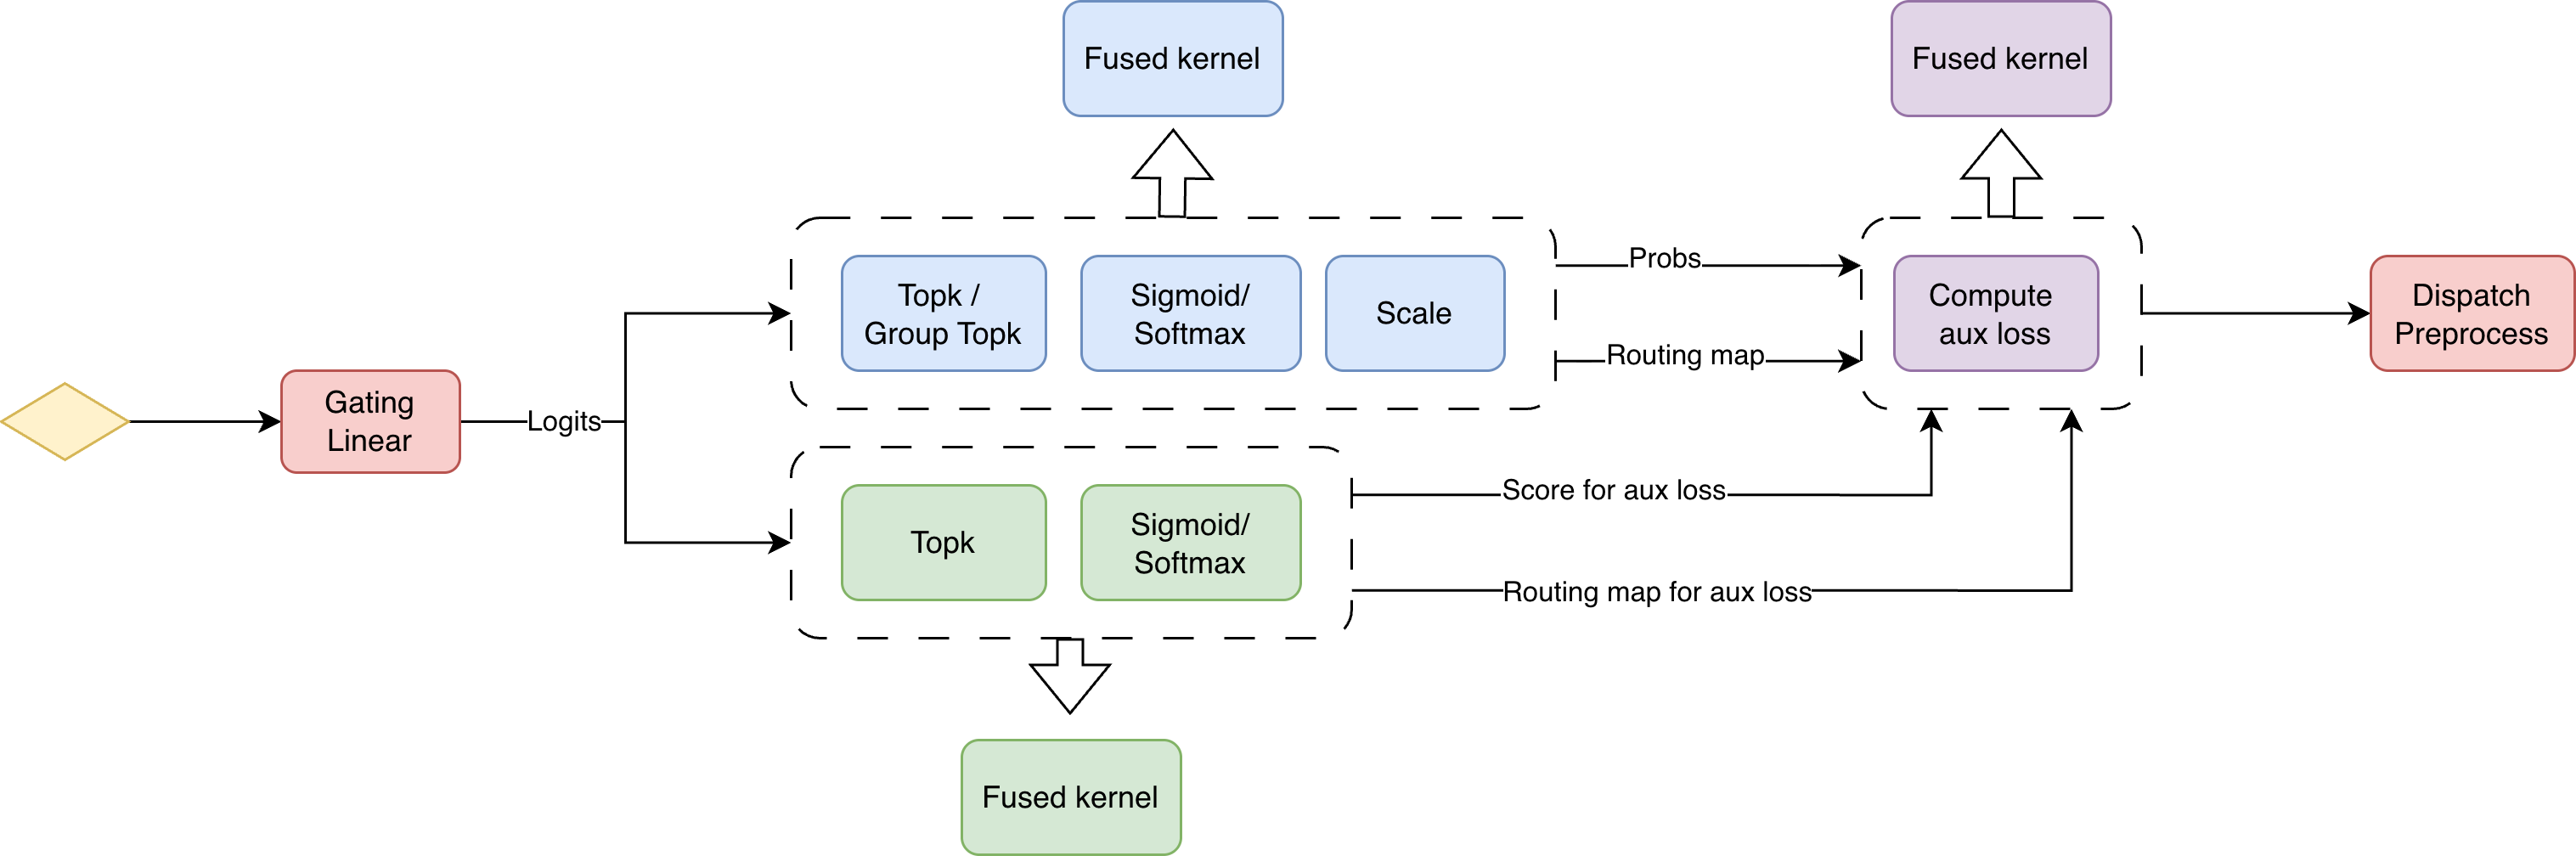
\includegraphics[width=1\linewidth]{figures/router_fusion.drawio.png}
    \caption{The workflow of the router fusion.}
    \label{fig:router_fusion}
\end{figure}
\begin{itemize}
    \item Score computation, including top-$k$ and softmax/sigmoid: This is the most complex function, with various branches for different models. It includes different top-$k$ algorithms (naive top-$k$, group top-$k$ \cite{deepseekai2024deepseekv2strongeconomicalefficient,deepseekai2025deepseekv3technicalreport}), score functions (sigmoid, softmax), their combinations, and possible scaling operations.
    \item Score computation for auxiliary loss: This is a subset of the first section. After the score function and naive top-$k$ computation, the input for auxiliary loss calculation is generated.
    \item Computation of MoE auxiliary loss: Building on step 2, the auxiliary loss computation is fused into a single kernel.

\end{itemize}
After enabling router fusion, the workflow within the router module is shown in \figref{fig:router_fusion}. Future work may incorporate communication into the fusion scope.

\subsubsection{Reduced-Precision Training: Low-Precision Acceleration}\label{sec:fp8-training}

Fine-grained MoE workloads with small expert GEMMs are often memory-bandwidth bound, limiting Tensor Core utilization. Reduced-precision training addresses this issue by reducing data movement and using faster FP8/FP4 Tensor Core operations on Hopper and Blackwell GPUs.

From a computation efficiency perspective, reduced-precision training provides a key benefit: \textbf{FP8/FP4 GEMMs} maximize Tensor Core utilization by performing Linear Layer computation in FP8/FP4. Together with the memory benefits in Sections~\ref{sec:fp8-activation}, FP8 training achieves approximately \textbf{10\% to 25\% end-to-end performance improvement} for large-scale MoE training on different hardware platforms, while FP4 gives it even more speedup.

For complete coverage of reduced-precision training recipes, MoE-specific challenges, and quantization strategies, see Section~\ref{sec:reduced-precision-training}.

\subsubsection{CUDA Graphs: Eliminating Host Overhead}\label{sec:cuda-graphs}

Kernel fusion reduces the \emph{number} of kernel launches; CUDA Graphs eliminate the \emph{per-iteration cost} of those launches. This subsection presents how CUDA Graphs address CPU overhead, the different strategies for drop-and-pad versus dropless MoE, and the memory optimizations required to make CUDA Graphs practical.

In MoE training, CPU overhead often becomes the dominant performance bottleneck. This overhead stems from three sources:
\begin{enumerate}
    \item \textbf{Python execution}: Interpreter overhead, C foreign function interface (CFFI), and garbage collection introduce latency.
    \item \textbf{Framework overhead}: Even simple operations such as \texttt{torch.empty} add microseconds of host-side cost; library layers (TransformerEngine, cuBLAS, cuDNN) add more.
    \item \textbf{Kernel launch overhead}: Each kernel launch incurs several microseconds of CPU-side cost.
\end{enumerate}

Three trends amplify this in modern training:
\begin{itemize}
    \item \textbf{Faster GPUs}: As kernel execution speeds increase, less time remains to overlap CPU work, making CPU overhead increasingly visible.
    \item \textbf{MoE complexity}: MoE models add substantial complexity to FFN layers---routers, dispatch, Grouped GEMMs, and combine operations---yielding many small kernels beyond the GEMMs themselves and thus substantial CPU overhead.
    \item \textbf{Reduced-precision training}: Extra quantization kernels, especially in fine-grained MoE where operation count scales with the number of experts.
\end{itemize}

\begin{figure}[ht]
    \centering
    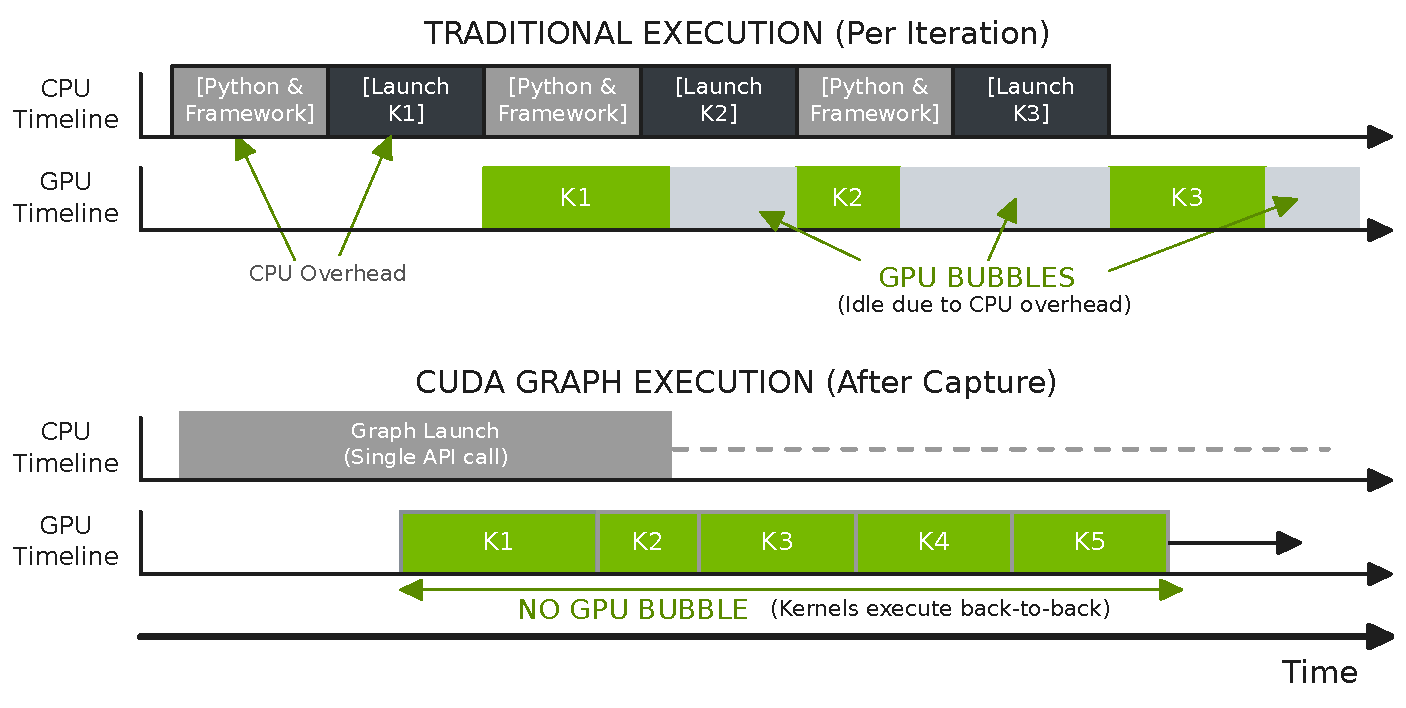
\includegraphics[width=0.8\textwidth]{figures/cuda_graph_comparison.pdf}
    \caption{Traditional execution (top) versus CUDA Graph execution (bottom).}
    \label{fig:cuda-graph-execution-comparison}
\end{figure}

% Nsight Systems profiling of non-CUDA Graph MoE training (the upper half of \figref{fig:partial_cudagraph_nsys}) 
\Figref{fig:cuda-graph-execution-comparison} shows the large CPU overhead and the resulting GPU bubbles in a traditional execution pipeline, revealing large gaps between GPU kernels. This clearly indicates that the CPU cannot launch kernels fast enough to keep the GPU fully utilized, a phenomenon known as CPU overhead or host-boundedness.
CUDA Graphs address this by capturing a sequence of GPU kernels into a replayable graph during an initial iteration \cite{nvidia_cudagraphs,ansel2024pytorch2}. Subsequent iterations issue a single \textit{Graph Launch} call, largely bypassing per-op Python/framework overhead and per-kernel launch overhead, thereby reducing CPU-side latency.

However, CUDA Graphs require all captured operations to have \textbf{static, predetermined shapes}. Dynamic shapes or control flow cause graph capture to fail. This creates a fundamental tension with MoE, where token counts per expert vary dynamically. The next paragraph describes Megatron-Core's two CUDA Graph modes---full CUDA Graphs and layer-wise CUDA Graphs---and how they address this dynamic-shape constraint in MoE.

\begin{figure}[ht]
    \centering
    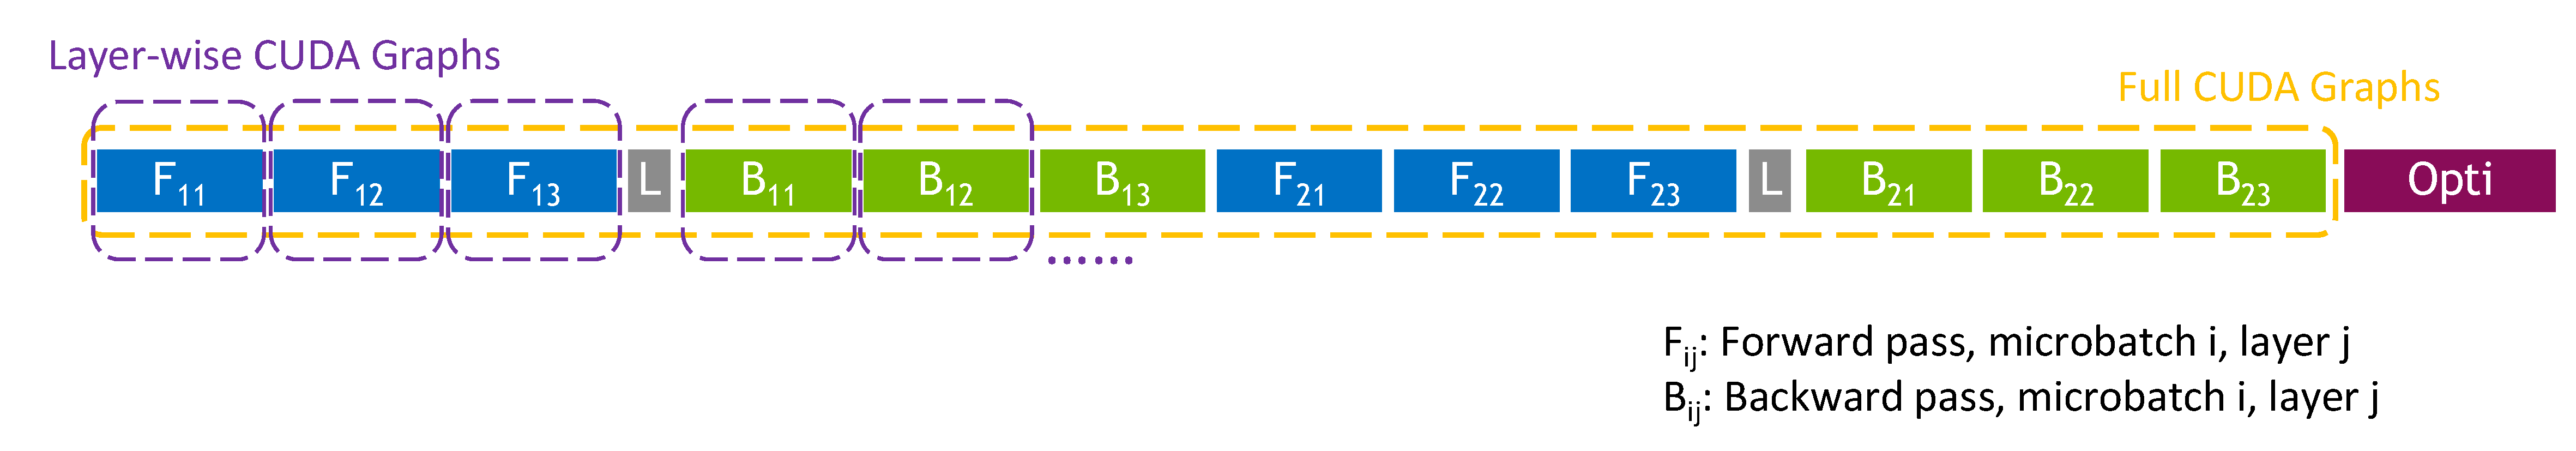
\includegraphics[width=0.95\linewidth]{figures/full_iter_layerwise.pdf}
    \caption{Full versus layer-wise CUDA Graphs in one training iteration (three layers, two microbatches).}
    \label{fig:full_iter_layerwise}
\end{figure}

\paragraph{Full CUDA Graphs vs Layer-wise CUDA Graphs}

As shown in \figref{fig:full_iter_layerwise}, two types of CUDA Graphs are supported in Megatron-Core: full CUDA Graphs and layer-wise CUDA Graphs. \textit{Full} CUDA Graphs, also noted as full-iteration CUDA Graphs, capture the entire forward-backward pass into a single CUDA Graph. This is only supported for dense or MoE models using \textbf{token dropping with padding}, which means each expert has a fixed receiving capacity; tokens exceeding capacity are dropped, and inputs are padded to ensure constant tensor shapes. With all shapes static, the whole iteration can be graphed, maximizing CPU overhead reduction. As for \textbf{dropless} MoE models such as DeepSeek-V3, where no routed tokens can be dropped, full CUDA Graphs are not feasible because the number of tokens assigned to each expert varies dynamically based on routing decisions. Expert GEMM shapes change from iteration to iteration, violating the static-shape requirement. Additionally, \textit{device-host synchronization} is required to retrieve per-expert token counts for dispatching. Section~\ref{sec:sync-free-moe} describes our effort to overcome the dynamic dispatching and synchronization issues so that the full CUDA Graphs can also be applied to dropless MoE. Alternatively, here we introduce a simpler method based on layer-wise CUDA Graphs, called \textit{partial} CUDA Graphs.

\begin{comment}
Megatron-Core supports full-iteration CUDA Graph for drop-and-pad MoE models via the \texttt{local} implementation:

\begin{lstlisting}
--moe-expert-capacity-factor 1.0 \
--moe-pad-expert-input-to-capacity \
--cuda-graph-impl local \
--cuda-graph-scope full_iteration
\end{lstlisting}
\end{comment}

% Instead of capturing the entire forward-backward pass into a single CUDA Graph, layer-wise CUDA Graphs capture each transformer layer separately. Note that both full CUDA Graphs and layer-wise CUDA Graphs are natively \textbf{not feasible for dropless MoE models} such as DeepSeek-V3, where no routed tokens can be dropped, so the number of tokens assigned to each expert varies dynamically based on routing decisions. Expert GEMM shapes change from iteration to iteration, violating the static-shape requirement. Additionally, \textit{device-host synchronization} is required to retrieve per-expert token counts for dispatching. Section~\ref{sec:sync-free-moe} describes our effort to overcome the dynamic dispatching and synchronization issues so that the full CUDA Graphs (either the full-iteration CUDA Graphs or full-layer-wise CUDA Graphs) can also be applied to dropless MoE. Alternatively, here we introduce a simpler method based on layer-wise CUDA Graph, called partial CUDA Graphs, which selectively captures only the \textbf{static components} of each MoE layer while leaving dynamic parts outside the graph, achieving significant performance gains for dropless MoE despite not capturing the entire model.

\begin{figure}[ht]
    \centering
    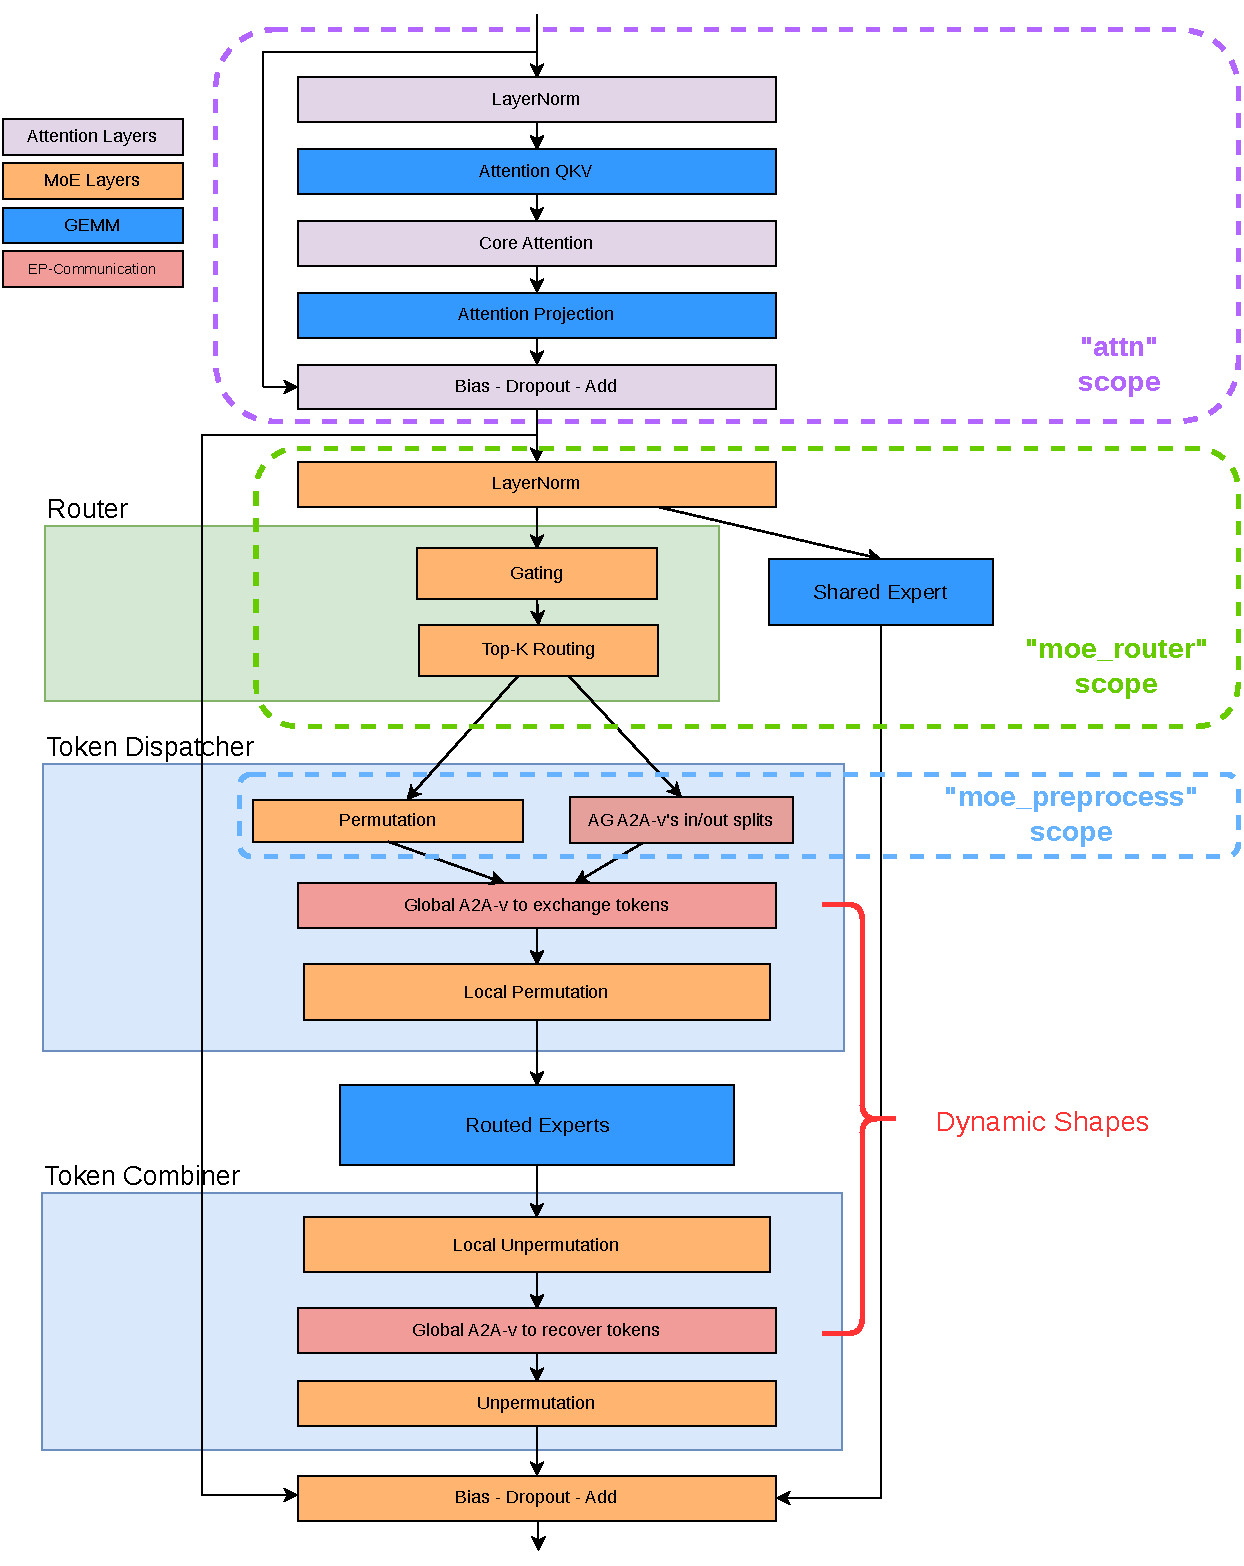
\includegraphics[width=0.6\linewidth]{figures/partial-cudagraph.pdf}
    \caption{Partial CUDA Graphs capture static components (attention, shared experts, router, preprocessing) while leaving dynamic expert computation outside the graph.}
    \label{fig:partial_cudagraph}
\end{figure}

Layer-wise CUDA Graphs capture each transformer layer separately. As with full CUDA Graphs, capturing an entire transformer layer still runs into dynamic shapes in the MoE part. Partial CUDA Graphs avoid this by capturing only the \textbf{static components} of each layer while leaving dynamic parts outside the graph, yielding large performance gains for dropless MoE even without capturing the full model. In a dropless MoE layer:

\begin{itemize}
    \item \textbf{Static components} (can be graphed):
    \begin{itemize}
        \item Attention layers (process a fixed number of tokens)
        \item Router computation (fixed input/output shapes)
        \item Expert Parallelism (EP) preprocessing (static permutation metadata)
        \item Shared experts (if present, process all tokens with fixed shapes)
        \item MLP layers in dense transformer blocks
    \end{itemize}

    \item \textbf{Dynamic components} (cannot be graphed):
    \begin{itemize}
        \item Token dispatch (from fixed shape to dynamic shape)
        \item Expert GEMM operations (dynamic M dimension based on token assignment)
        \item Token combine (from dynamic shape to fixed shape)
    \end{itemize}
\end{itemize}

Partial CUDA Graphs capture the static portions of each layer independently, leaving routed expert computation to execute normally.
As shown in \figref{fig:partial_cudagraph}, the forward path of each transformer layer is split into several ``scopes'', and the user can choose which scopes to graph. With the "\textit{attn+moe\_router+moe\_preprocess}" scopes enabled, one graph captures all static components before the dispatching operation for that layer: attention, router (projection, top-$k$ selection, and auxiliary loss computation), and EP preprocessing (token metadata calculation and permutation). A shared expert, if present, is also captured in this graph. This approach eliminates CPU overhead while preserving correctness by allowing dynamic expert computation to execute with varying shapes. Despite not capturing the entire model, this achieves significant performance gains.

\begin{figure}[ht]
    \centering
    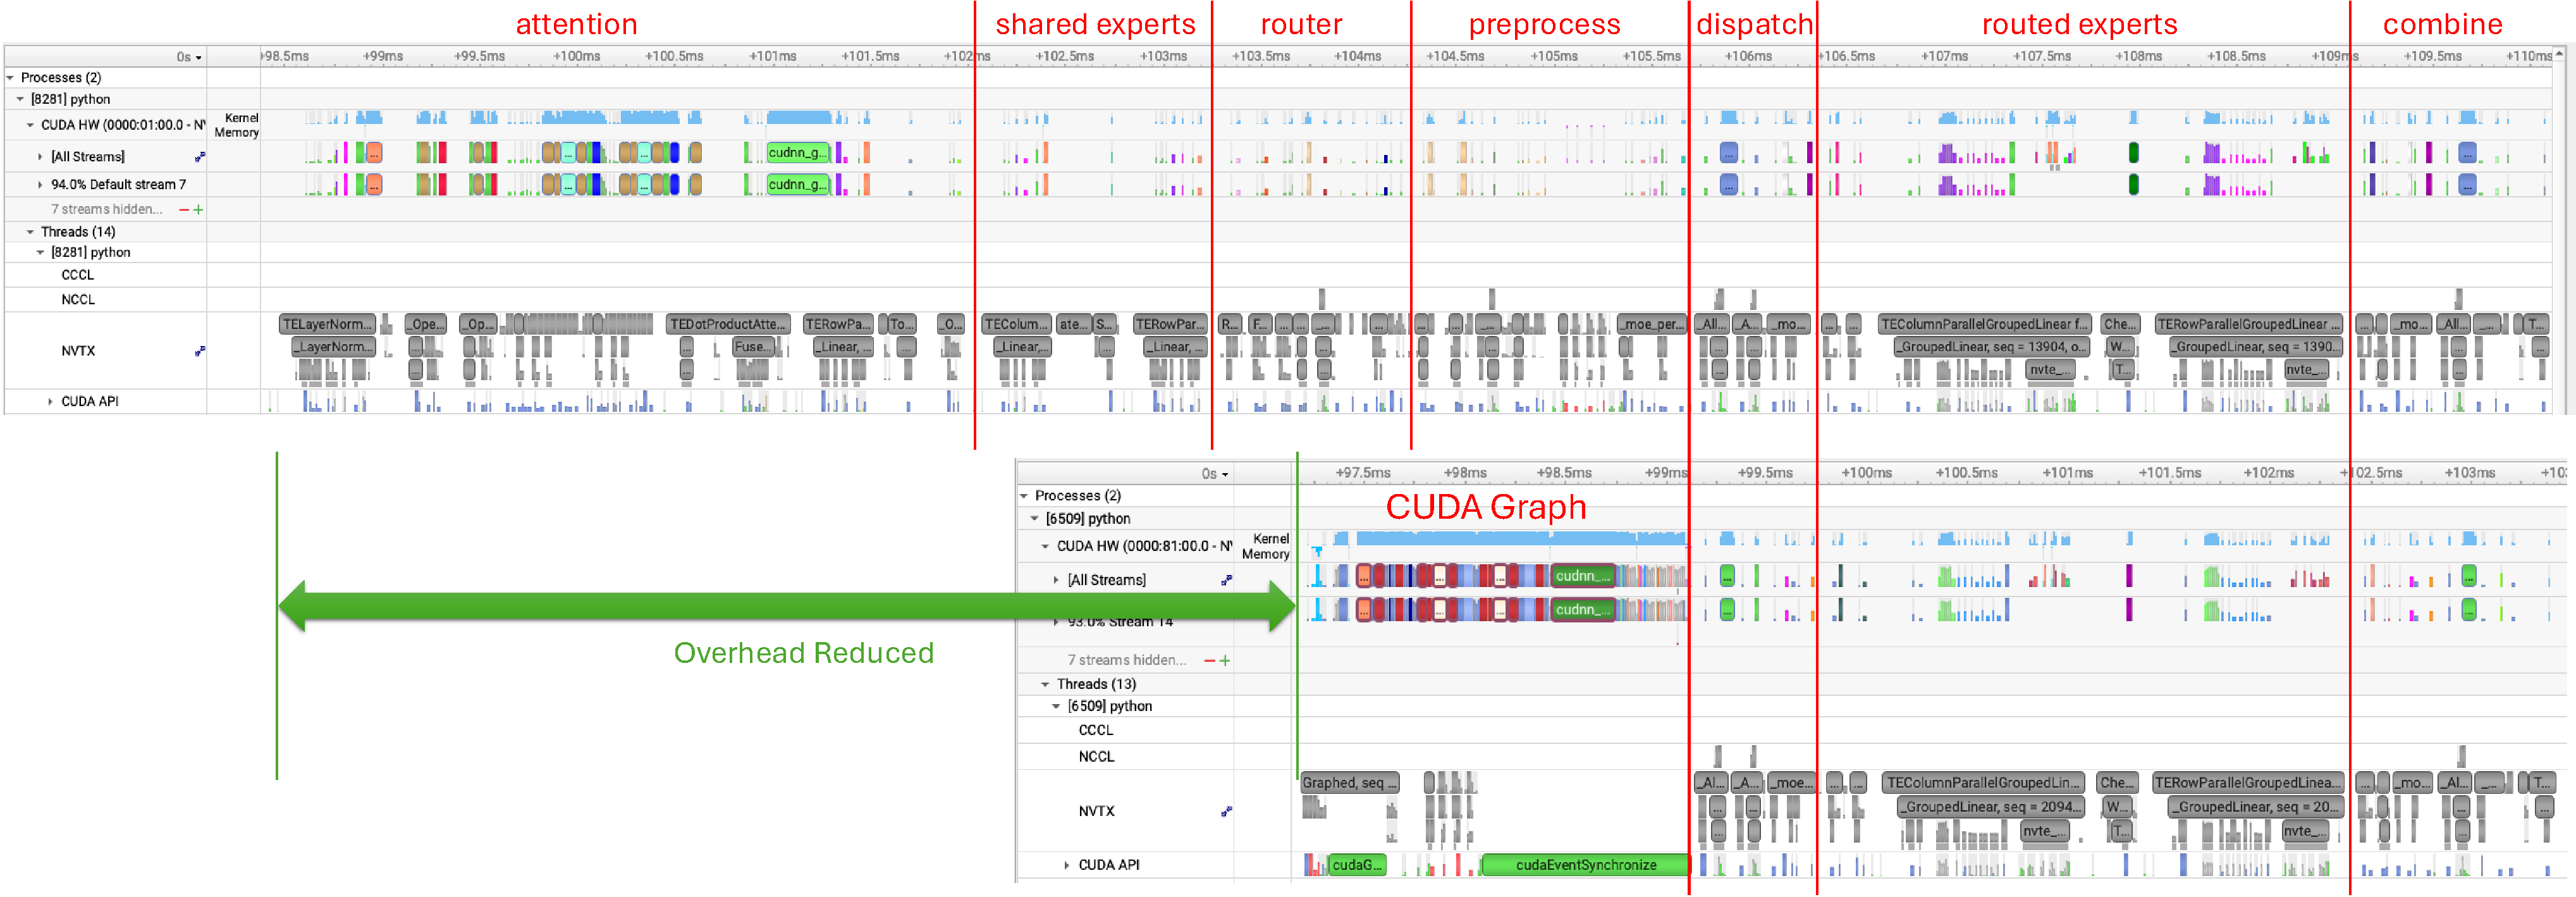
\includegraphics[width=0.95\linewidth]{figures/partial-cudagraph-nsys.pdf}
    \caption{Transformer layer forward pass: without (upper) and with (lower) partial CUDA Graphs. CPU overhead is largely eliminated for static components.}
    \label{fig:partial_cudagraph_nsys}
\end{figure}

Megatron-Core has been extensively adapted so that CUDA Graphs work correctly with key features like Multi-Token Prediction (MTP), EP communication overlapping, fine-grained offloading and checkpointing, and flexible PP layouts. Nsight Systems profiling with partial CUDA Graphs enabled shows greatly reduced CPU overhead (\figref{fig:partial_cudagraph_nsys}). The remaining CPU overhead is primarily confined to the region between token dispatch and combine operations, which cannot be graphed due to their dynamic nature. See Section~\ref{sec:sync-free-moe} for more details on how to address this remaining bottleneck by making the whole layer graphable.

\paragraph{Memory Optimizations for CUDA Graphs}

CUDA Graphs add memory overhead from three sources:

\begin{enumerate}
    \item \textbf{Graph structure}: Memory for storing the graph topology (typically negligible).
    \item \textbf{Separate memory pools}: Graphed and non-graphed operations need separate PyTorch memory pools and cannot share memory. With partial CUDA Graphs, a single transformer layer needs two pools: one for graphed work and one for non-graphed work.
    \item \textbf{Static buffers}: Each graph needs dedicated input/output static buffers that, once allocated, are taken out of PyTorch's memory allocator.
\end{enumerate}

If not carefully optimized, partial CUDA Graphs would incur much higher memory overhead from the above three sources. Megatron-Core and Transformer Engine implement several optimizations to minimize this overhead:

\textit{Reducing the number of graphs.}
With pipeline parallelism (PP), \textbf{each microbatch} requires a dedicated CUDA Graph. The reason is that if microbatches share a graph, microbatch $i+1$'s forward pass will overwrite the saved context before microbatch $i$'s backward pass executes, causing memory corruption (\figref{fig:pp-microbatch-graph-sharing}). This results in $L \times M \times 2$ graphs in total (where $L$ = layers per GPU, $M$ = microbatches, $\times 2$ for forward/backward).

On the contrary, if PP is not used, microbatches can share the same graph, reducing the count to $L \times 2$. To enable graph sharing, an \texttt{is\_first\_microbatch} GPU flag is introduced to control microbatch-specific behaviors within the shared graph, e.g., quantization that runs only on the first microbatch. Setting this flag to 0 or 1 before replay causes the captured quantization kernel to be skipped or executed as needed.

\begin{figure}[ht]
    \centering
    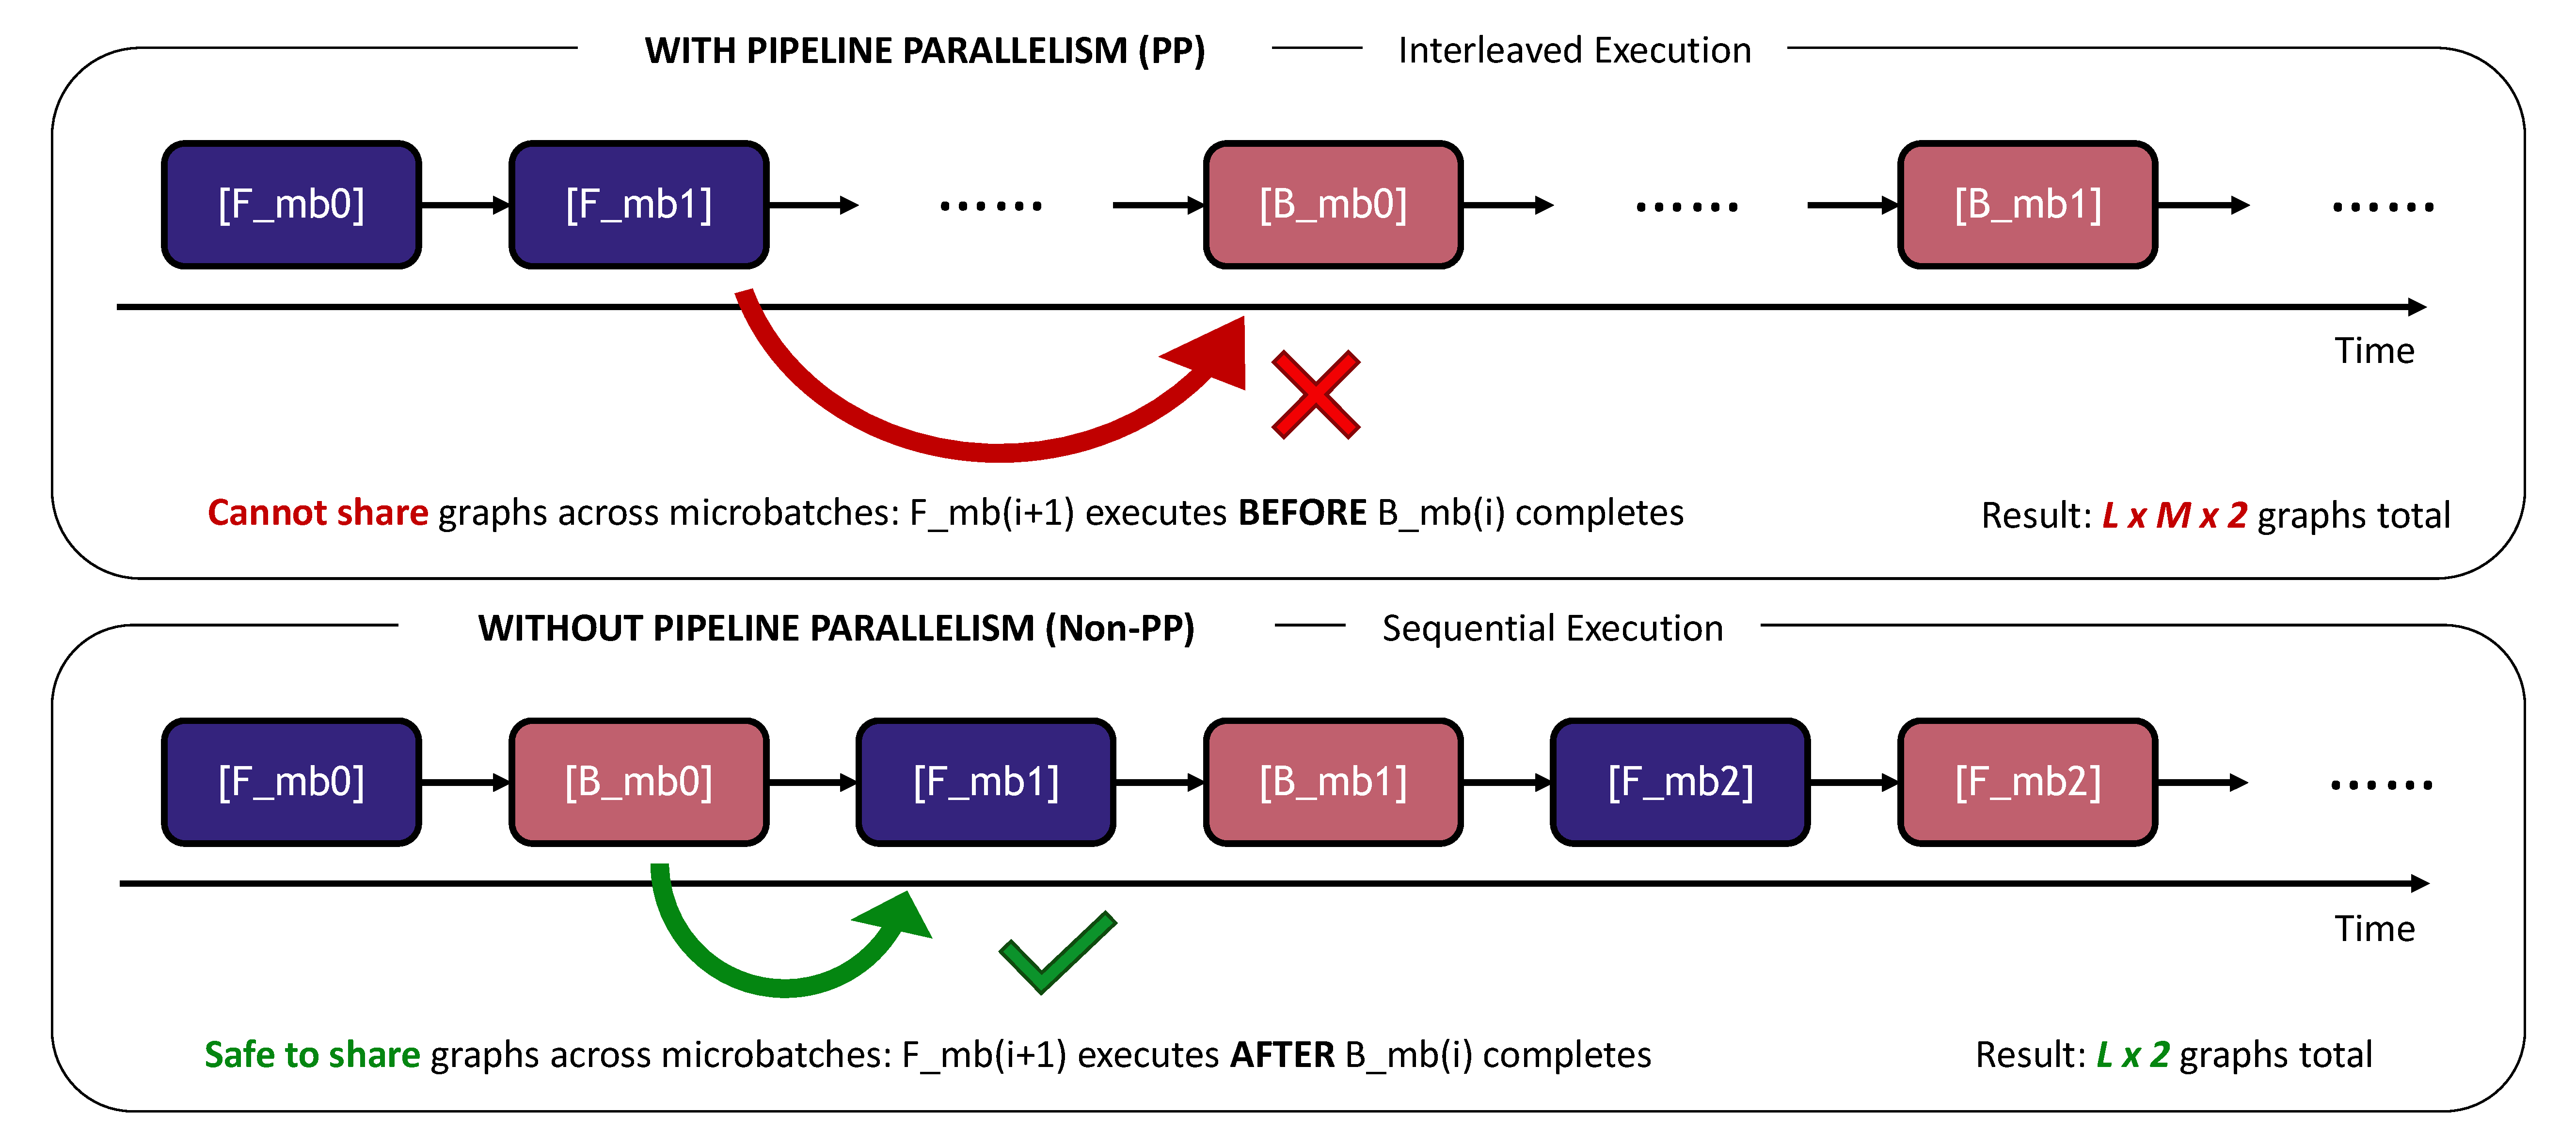
\includegraphics[width=0.9\textwidth]{figures/cudagraph_pp.pdf}
    \caption{Why Pipeline Parallelism prevents CUDA Graphs from being shared across microbatches. \textbf{With PP} (top): Execution is interleaved---multiple forward passes run before any backward pass. If microbatches share a graph, F\_mb1 overwrites saved context of F\_mb0 before B\_mb0 uses it, causing memory corruption. Each microbatch needs its own graph ($L \times M \times 2$ graphs total). \textbf{Without PP} (bottom): Execution is sequential---each microbatch completes (forward+backward) before the next starts. Context is consumed before being overwritten, so microbatches can safely share graphs (only $L \times 2$ graphs total).}
    \label{fig:pp-microbatch-graph-sharing}
\end{figure}

\textit{Pool sharing.}
Although graphed and non-graphed operations require separate memory pools, all graphs can share one pool when captured in execution order. Transformer Engine's \texttt{make\_graphed\_callables()} API accepts an \texttt{\_order} argument that specifies the inter-microbatch scheduling, allowing sequential capture with correct pool sharing.

\textit{Buffer reuse.}
Static input/output buffers can be reused across graphs according to the PP execution order. Once a microbatch finishes its backward pass of a layer, its forward buffers and backward input buffer become available for the next forward and backward graphs to reuse. Only the backward output buffer must be kept until the data is sent to the next PP stage.

With these memory optimizations, we achieve 10\% end-to-end speedup with about 7~GB extra memory on DeepSeek-V3 GB200 training.

\paragraph{The Remaining Problem: Dynamic Expert Computation}

Full CUDA Graphs do not support dropless MoE. Partial CUDA Graphs eliminate CPU overhead for static components, but \textbf{the dynamic expert computation region remains outside the graph}. Is there any way we could make CUDA Graphs \textit{cover} the dynamic part? There are at least two challenges we must solve to achieve this:
\begin{enumerate}
    \item \textbf{Dynamic shapes require host--device synchronization}: The host must query per-expert token counts from the GPU to launch token dispatching and Grouped GEMMs.
    \item \textbf{Memory allocation requires known buffer sizes}: Worst-case buffer allocation wastes memory; actual-size allocation requires synchronization.
\end{enumerate}

The next subsection presents how Megatron-Core achieves full CUDA Graphs coverage for dropless MoE through three complementary techniques: sync-free kernels, ECHO, and Paged Stashing.

\subsubsection{Full CUDA Graphs Coverage for Dropless MoE via Sync-Free Kernels, ECHO, and Paged Stashing}\label{sec:sync-free-moe}

While kernel fusion and CUDA Graphs help reduce host overhead, dropless MoE introduces a new challenge: dynamic tensor shapes require host-device synchronization, preventing CUDA Graphs from covering expert computation.

In dropless MoE, token counts received by each EP rank vary dynamically based on routing decisions. The router generates this shape information on the GPU, but the host needs it to launch subsequent operations and allocate memory. Obtaining this information requires a device-to-host copy and synchronization, placing the CPU on the critical path and preventing CUDA Graphs capturing of the dynamic portions. To enable sync-free MoE for dropless training with dynamic routing, there are two fundamental challenges:

\textbf{Challenge 1: Kernel launch without knowing the actual problem size.}
Conventionally, many GPU operators assume that (dynamic) shape information is available on the host. The host-side code determines launch configurations, such as grid size and tile size, as well as the amount of work the kernel must perform based on the shape information obtained at run time. In dropless MoE, this creates a host-device synchronization point: the host must query per-expert token counts from the device before launching Grouped GEMM or communication kernels. To tackle this issue, the GPU kernels handling dynamic shapes need to be redesigned. We developed \textbf{device-initiated GPU kernels}, including device-initiated Grouped GEMM and sync-free dispatch with HybridEP.

\textbf{Challenge 2: Memory allocation without knowing the actual size.}
Sync-free execution means the size of buffers needs to be pre-determined on the host. To avoid token overflow, buffers often need to be over-sized, e.g., based on the worst-case size to accommodate the case where all tokens are routed to the same expert. This over-provisioning, however, leads to severe memory fragmentation: if the actual token distribution is balanced, the vast majority of the preallocated memory remains unused, yet it cannot be reclaimed by other operations within the graph. The worst-case buffer potentially requires $O(\text{EP\_size})$ times more memory than the actual working set.

This memory fragmentation can be mitigated through two complementary strategies: \emph{reducing load imbalance} so that worst-case provisioning is closer to actual usage, and \emph{dynamic memory management} within the CUDA Graph to reclaim unused buffer space. \textbf{ECHO} employs the first strategy by dynamically cloning popular experts on underutilized ranks, reducing the variance in per-rank token counts and thus the gap between worst-case and average memory requirements. \textbf{Paged Stashing} adopts the second strategy by enabling fine-grained memory management within CUDA Graph, allowing unused portions of preallocated buffers to be repurposed for other operations. ECHO and Paged Stashing are detailed below.

\paragraph{Device-Initiated GPU Kernels}
\label{sec:device-init}

To eliminate the mandatory host-device synchronization required by conventional host-initiated GPU operators, kernels must be \emph{device-initiated}. This requires three things:
\begin{itemize}
\item[i.] The GPU kernel needs to read shape information from GPU memory and use it to guide the computation.
\item[ii.] The GPU kernel needs to decouple the actual amount of work it performs, which is only known at runtime, from its static launch configuration.
\item[iii.] The GPU kernel needs to skip unnecessary computation, such as operations on padded data.
\end{itemize}
To satisfy these requirements, existing kernels must be redesigned. The Grouped GEMM kernel and HybridEP kernel serve as two concrete examples below.

\textbf{Device-Initiated Grouped GEMM.}
As discussed in Section~\ref{sec:grouped-gemm}, TE offers two Grouped GEMM implementations: the multi-stream cuBLASLt GEMMs and the CUTLASS Grouped GEMM. Both are host-initiated. They require a CPU-side list of per-expert token counts to determine each GEMM's shape and launch configuration, creating a host-device synchronization barrier. To eliminate this, TE introduces device-initiated Grouped GEMM, which reads shape information directly from device memory. Two implementations are provided:

\begin{itemize}
\item[i.] \textbf{cuBLASLt Grouped GEMM.}
Since CUDA 13.1, cuBLASLt Grouped GEMM supports passing matrix shapes as device arrays. This implementation includes built-in heuristics for selecting optimal kernel configurations, now covering various precisions and scaling modes across recent CUDA releases.

\item[ii.] \textbf{cuteDSL Grouped GEMM with Fused Activation and Quantization.}
In the cuteDSL-based implementation, the SwiGLU activation can be fused into the epilogue stage, and for FP8 training, quantization can also be fused. While current support is limited to specific precisions and fusion patterns, ongoing development continues to expand coverage across new configurations.
\end{itemize}

\textbf{Sync-Free Dispatch with HybridEP.}
HybridEP, introduced in Section~\ref{sec:deepep}, provides an efficient implementation of MoE communication and also plays an important role in sync-free MoE. After each dispatch and permutation, the number of tokens received by a given rank is dynamic, normally requiring synchronization to obtain buffer sizes. By estimating an upper bound and passing it to HybridEP, the dispatcher can pre-allocate output buffers according to this bound, eliminating all synchronizations at the cost of additional GPU memory.

Even with device-initiated kernels, worst-case buffer allocation wastes memory. Two complementary strategies address this: \textbf{ECHO} reduces load imbalance so worst-case provisioning approaches actual usage, while \textbf{Paged Stashing} enables fine-grained memory management to reclaim unused buffer space.

\paragraph{ECHO: Elastic Cloning for Hot Experts.}\label{sec:echo}\footnote{Implementation details: \url{https://github.com/NVIDIA/Megatron-LM/pull/2368}}

Load imbalance is inherent in MoE: popular experts receive far more tokens than others, creating two problems. First, EP ranks hosting hot experts become compute bottlenecks, causing other ranks to wait at synchronization points. Second, high load variance means worst-case buffer provisioning wastes significant memory compared to actual usage. ECHO addresses both by dynamically cloning hot experts to spare slots on underutilized ranks.

\figref{fig:echo} illustrates the ECHO workflow. In the forward pass, the ECHO planner identifies hot experts and generates two outputs: a \emph{hot expert map} indicating which experts to clone to which spare slots, and an updated \emph{routing map} redirecting overflow tokens to clones. Expert Dispatch copies hot expert weights to spare slots via HybridEP-based sync-free communication; Token Dispatch routes tokens to both home and cloned experts; expert computation proceeds on all experts. In the backward pass, Expert Gradient Dispatch collects gradients from clones and reduces them to home experts, ensuring consistency. Cloned experts are discarded after computation to save memory.

\begin{figure}[ht]
    \centering
    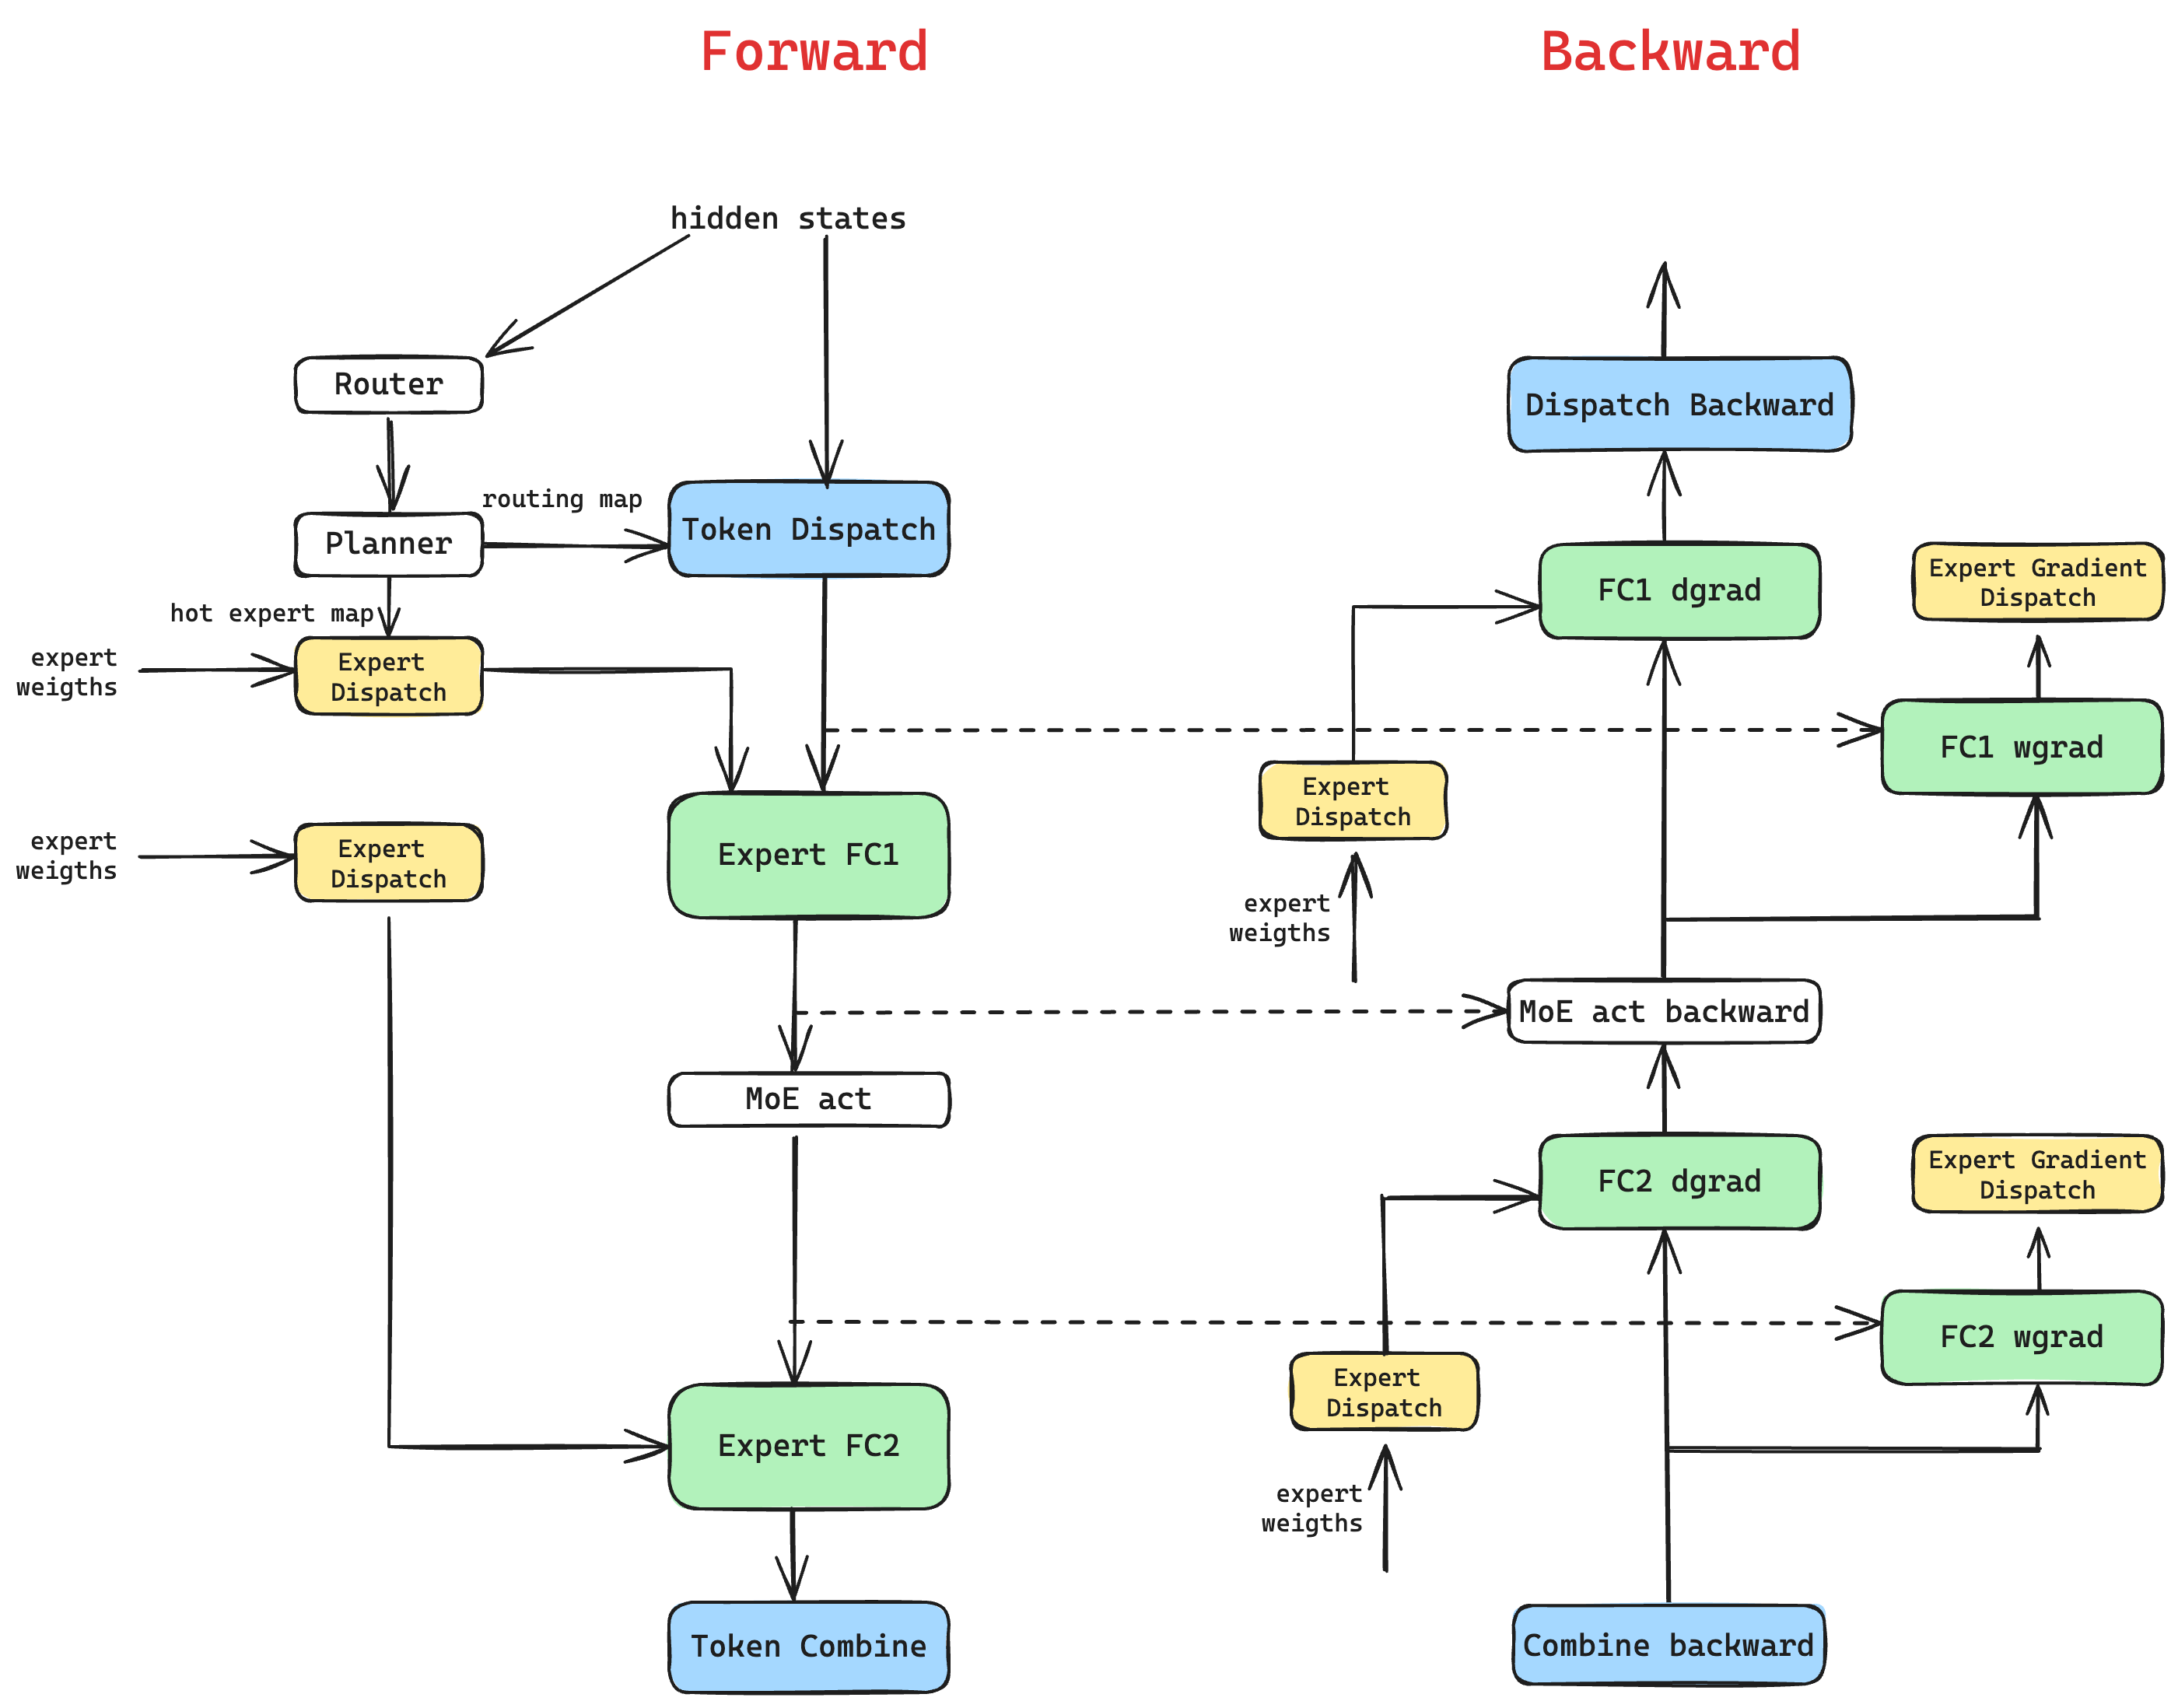
\includegraphics[width=0.85\linewidth]{figures/moe_echo.png}
    \caption{ECHO workflow for forward and backward passes. The planner generates routing and hot expert maps. Expert Dispatch clones hot expert weights to spare slots; Expert Gradient Dispatch reduces gradients back to home experts.}
    \label{fig:echo}
\end{figure}

Cloning experts for training is much more expensive than for inference: each cloned expert requires weight communication during forward and gradient reduction during backward to ensure consistency. Cloning all hot experts to all spare slots would maximize load balance but introduce excessive communication overhead. The goal of the ECHO planner is to minimize the number of expert clones while achieving sufficient load balance. It computes the \emph{spillover} for each expert (tokens exceeding the average load per EP rank) and the \emph{spare capacity} on each rank (available capacity below average). Using a bin-packing algorithm, the planner efficiently matches spillover tokens to spare capacity, determining which specific experts to clone and to which ranks, producing the hot expert map and routing map with minimal cloning overhead.

ECHO provides two key benefits: (1) \emph{reduced memory fragmentation for CUDA Graphs}, since reducing load variance across EP ranks makes worst-case buffer sizing closer to actual usage, enabling smaller static buffers; and (2) \emph{improved compute efficiency}, since balanced workloads reduce the straggler problem, improving overall GPU utilization.

\paragraph{Paged Stashing.}\footnote{Implementation details: \url{https://github.com/NVIDIA/Megatron-LM/pull/2690}}

While ECHO reduces load imbalance to narrow the gap between worst-case and typical memory requirements, Paged Stashing addresses the complementary problem: enabling fine-grained memory management within CUDA Graph to reduce internal memory fragmentation.

The fragmentation problem arises because sizes of buffers involved in CUDA Graphs need to be pre-determined. To avoid undesired overflow, the buffers usually need to be over-sized. In a straightforward approach, buffers in all layers are allocated according to the worst-case size (\figref{fig:paged_stash}, middle). For dropless MoE, this means each layer reserves a buffer based on maximum possible tokens each rank may receive, resulting in $O(\text{layers} \times \text{worst\_case})$ memory overhead even when actual token counts are much lower.

Paged Stashing is based on a key observation: there is a vast gap (often more than an order of magnitude) between the actual memory needed to store activations for backward computation and the worst-case memory allocated to avoid overflow at each layer. Paged Stashing addresses this by decoupling these two memory buffers. This is illustrated in \figref{fig:paged_stash} (right). Instead of allocating worst-case-sized buffers for every layer, the paged-stashing manager maintains: (1) a single \emph{tmp buffer} sized for the worst-case token counts, which is shared across all layers for computation, and (2) a \emph{stashing buffer} organized in the form of pages that stores only the actual tokens used by each layer. When a layer completes its forward computation, its activations are copied from the tmp buffer to the stashing buffer, storing only the actual token count rather than the worst-case allocation. The tmp buffer can then be readily reused for the computation in following layers. This significantly reduces memory consumption from $O(\text{layers} \times \text{worst\_case})$ to $O(\text{worst\_case} + \text{actual\_total})$.

\begin{figure}[ht]
    \centering
    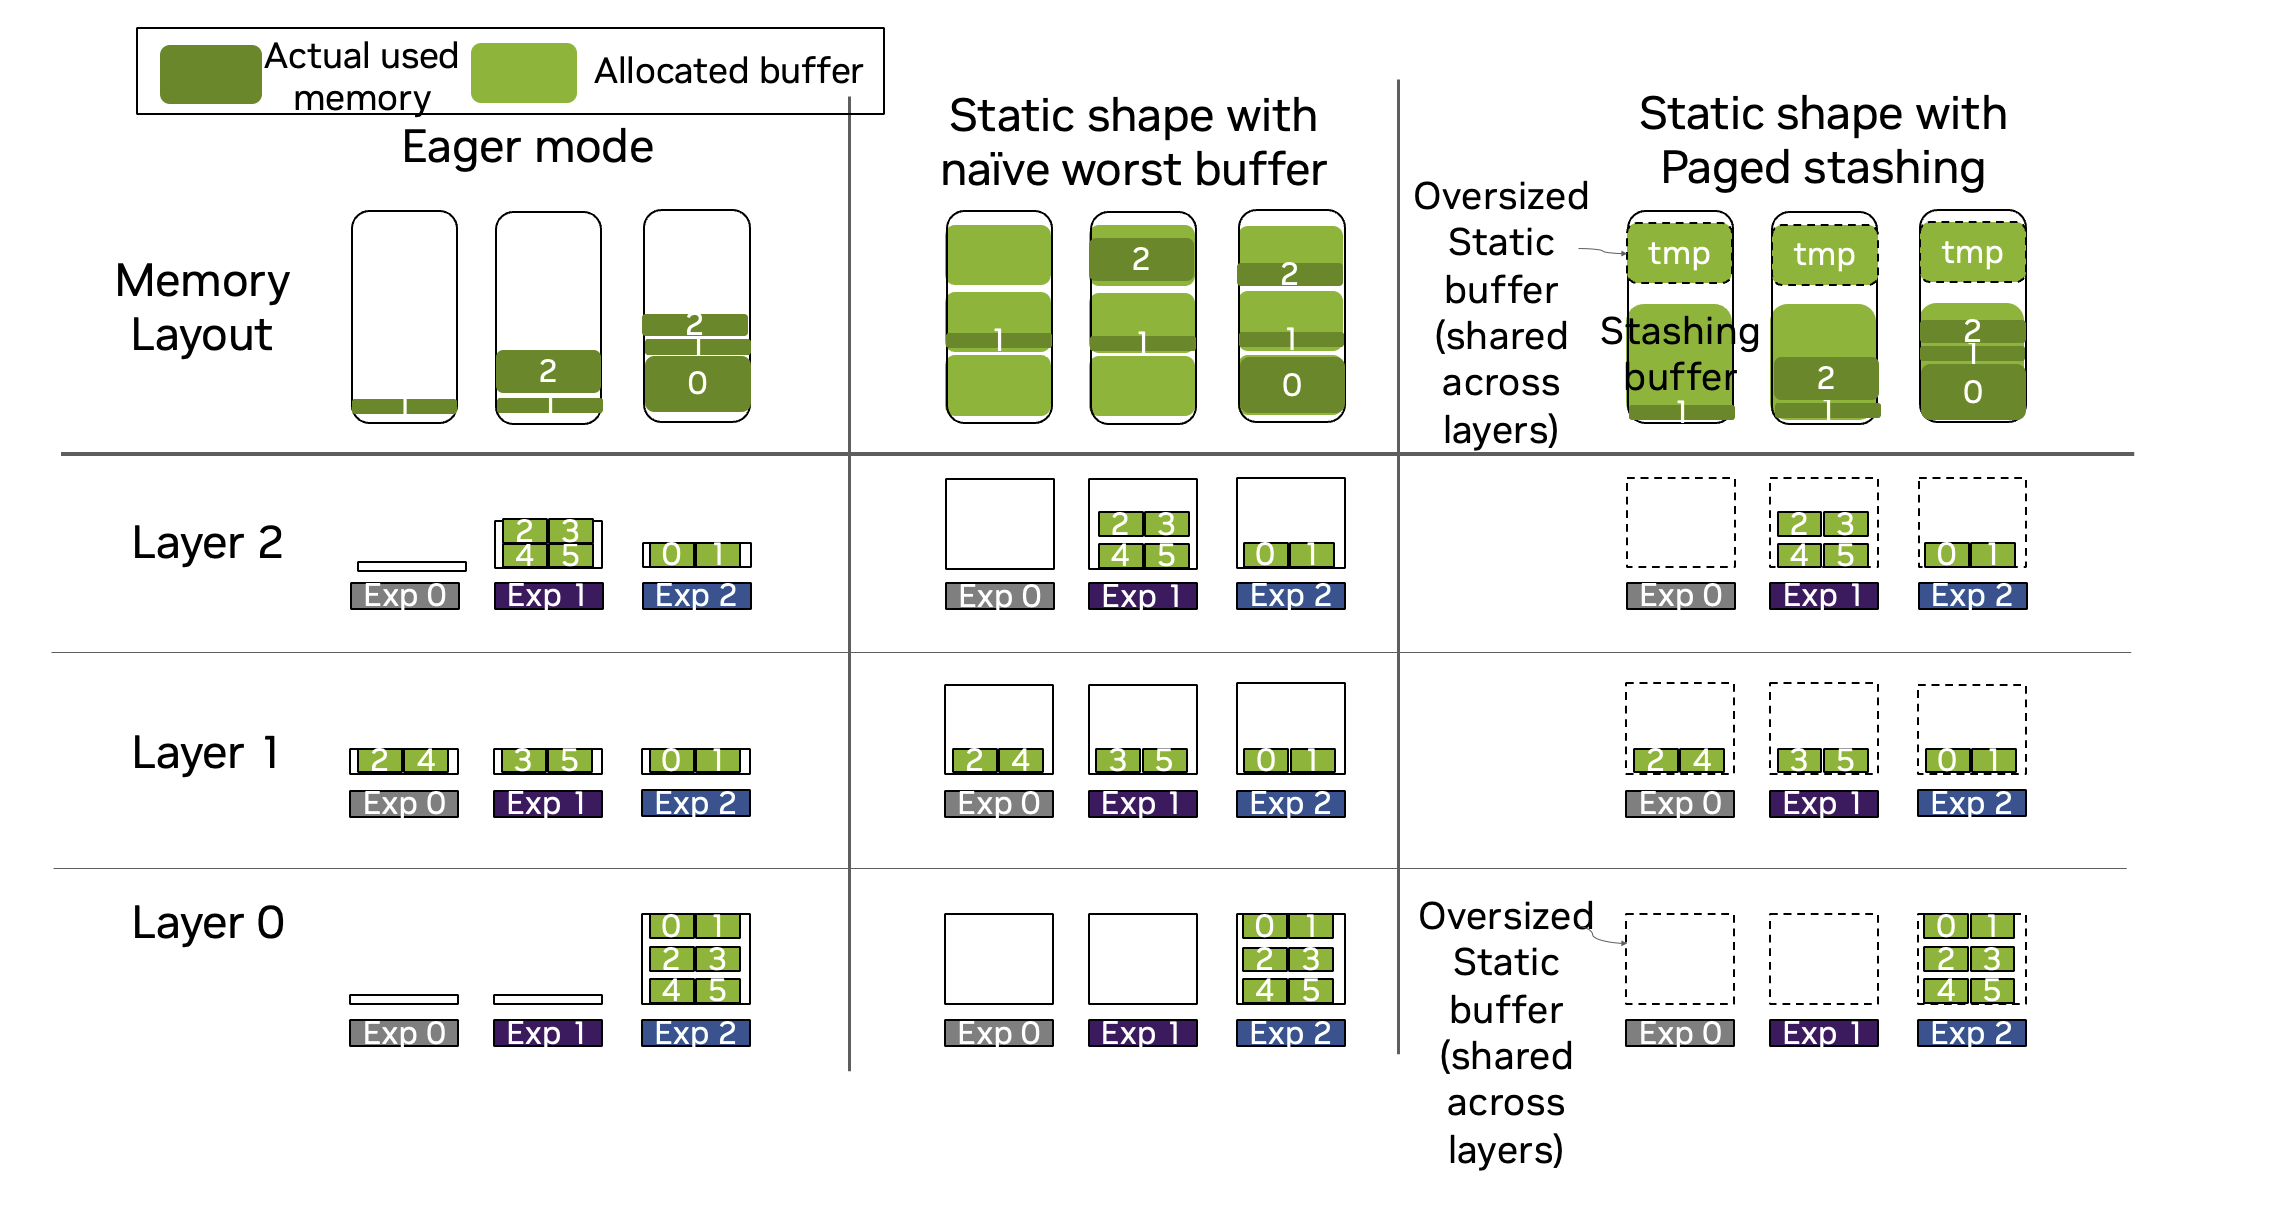
\includegraphics[width=0.95\linewidth]{figures/paged_stash.png}
    \caption{Memory layout comparison across three execution modes. \textbf{Left}: Eager mode allocates memory dynamically based on actual usage. \textbf{Middle}: Baseline static shape requires worst-case sized buffers for each layer independently, causing severe fragmentation when actual usage is lower. \textbf{Right}: Paged Stashing uses a single worst-case tmp buffer shared across layers for computation, while a paged stashing buffer stores only the actual tokens, significantly reducing total memory footprint.}
    \label{fig:paged_stash}
\end{figure}

The stashing buffer uses the classic idea of paging to manage memory in a flexible yet efficient way. The \texttt{PagedStashBuffer} is organized as pages of fixed size (default 64 tokens per page). The page stashing manager tracks available pages through a free list implemented by a circular buffer. Paging operations are implemented as device-initiated \emph{stash kernels}. The stash kernel copies activations to free pages allocated from the head of the free list and records the target pages. The \emph{reload kernel} retrieves activations from the recorded pages and returns the unused pages to the tail of the free list.

To minimize overhead, Paged Stashing overlaps memory transfers with computation using dedicated CUDA streams (\figref{fig:paged-stashing-overlap}). The system pre-fetches activations for the next backward layer while current computation executes, hiding reload latency. This overlap requires slight memory overhead due to double buffering.

\begin{figure}[ht]
    \centering
    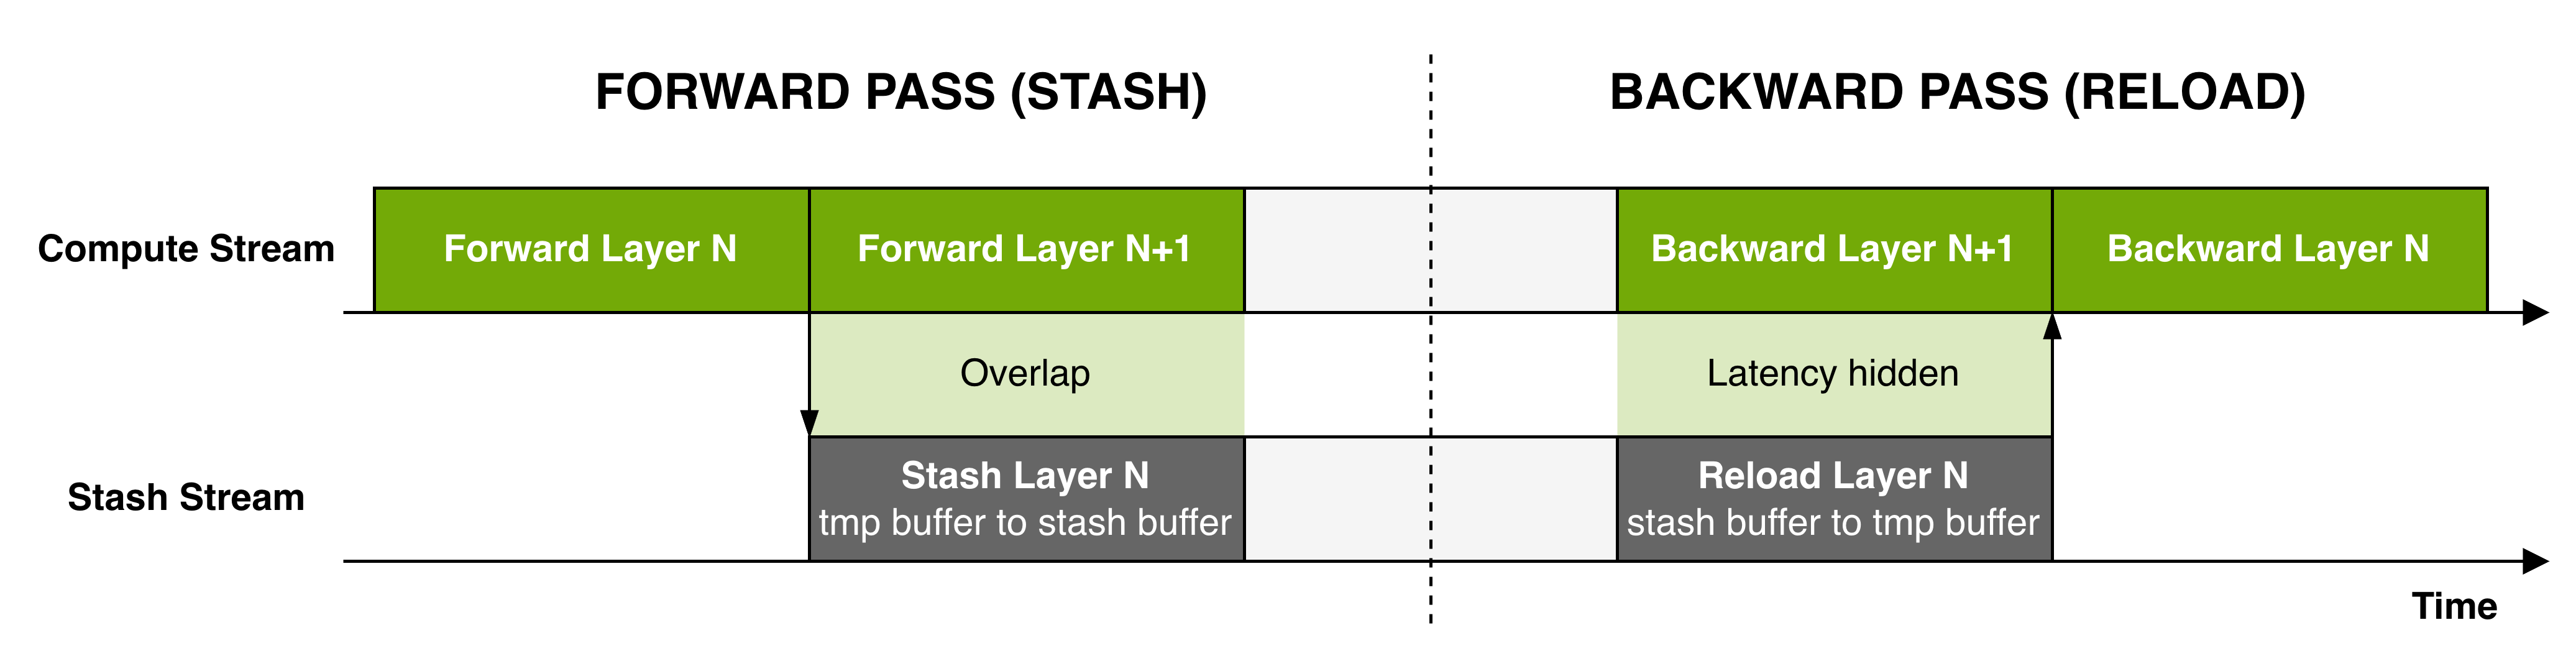
\includegraphics[width=0.9\textwidth]{figures/paged_stashing_overlap.drawio.png}
    \caption{Paged Stashing stream overlap. \textbf{Forward pass}: After Layer N computes, its activations are stashed (copied from tmp buffer to paged stashing buffer) on a dedicated Pack stream while Layer N+1 computes on the main Compute stream---the stash is completely overlapped. \textbf{Backward pass}: Activations for Layer N are pre-fetched (reloaded from stashing buffer to tmp buffer) on the Unpack stream before Layer N backward starts, hiding reload latency.}
    \label{fig:paged-stashing-overlap}
\end{figure}

\paragraph{Putting It Together: Full CUDA Graphs Coverage}

Together, these three techniques enable full CUDA Graphs coverage for dropless MoE, eliminating CPU overhead while preserving the flexibility of dynamic routing:
\begin{itemize}
    \item \textbf{Device-initiated kernels} remove host-device synchronization entirely by reading dynamic shapes directly from GPU memory, making all MoE operations capturable by CUDA Graphs.
    \item \textbf{ECHO} balances expert workloads across EP ranks, narrowing the gap between worst-case and actual buffer requirements. This enables smaller static allocations and mitigates the straggler problem that otherwise limits GPU utilization.
    \item \textbf{Paged Stashing} reduces memory from $O(\text{layers} \times \text{worst\_case})$ to $O(\text{worst\_case} + \text{actual\_total})$ by sharing a single worst-case tmp buffer across layers and storing only actual activations in a paged stashing buffer.
\end{itemize}

\noindent\textbf{Overhead.}
These benefits come with measured trade-offs.
ECHO introduces extra communication for cloning hot experts in the forward pass and reducing their gradients in the backward pass; in practice, only a small fraction of experts are cloned (determined by the spillover above average load), so the additional communication remains modest relative to the standard all-to-all dispatch.
Paged Stashing adds memory copy operations (stash in the forward pass, reload in the backward pass) and a persistent worst-case-sized tmp buffer with double-buffering overhead; these copies run on dedicated CUDA streams overlapped with layer computation, so the latency is largely hidden and the primary cost is additional memory bandwidth.
Both overheads are relatively small compared to the gains from eliminating per-iteration host-device synchronization and enabling static memory planning with CUDA Graphs.

\subsubsection{Summary}

The compute efficiency optimizations address both sources of inefficiency. For kernel efficiency: Grouped GEMM batches expert computations, kernel fusion consolidates routing and permutation operations, and reduced-precision training accelerates Tensor Core throughput. For host overhead: CUDA Graphs eliminate per-iteration CPU logic, and Sync-Free MoE removes host-device synchronization barriers. ECHO addresses load imbalance that compounds both issues. Together, these optimizations transform compute inefficiency from a dominant bottleneck into a manageable constraint.

